\documentclass[12pt]{article}

%-------------------------------------------------------------------------------
% PACKAGES
%-------------------------------------------------------------------------------
\usepackage[french, english]{babel}
\usepackage[utf8]{inputenc}
\usepackage[super]{natbib}
\usepackage{mathtools}
\usepackage{nameref}
\usepackage{fancyref}
\usepackage[margin=0.7in]{geometry}

% section numbering
%\makeatletter
%\def\@seccntformat#1{%
%  \expandafter\ifx\csname c@#1\endcsname\c@section
%  \fi}
%\makeatother

% diagrams
\usepackage{tikz}
\usetikzlibrary{shapes,arrows,shadows}
\usetikzlibrary{automata,positioning,arrows}
\usepackage{amsmath,bm,times}
\newcommand{\mx}[1]{\mathbf{\bm{#1}}} % Matrix command
\newcommand{\vc}[1]{\mathbf{\bm{#1}}} % Vector command

%figures
\usepackage{caption}
\usepackage{subcaption}
\usepackage{epstopdf}
\usepackage{graphicx}
\graphicspath{{pictures/}}
\epstopdfsetup{outdir=pictures/}

%fancy stuff like color, paragraph formatting, code
\usepackage{hyperref}
\hypersetup{
     colorlinks   = true,
     citecolor    = darkgray
}
\usepackage{amsthm}
\usepackage{enumitem}
\setlist{nosep}
\usepackage{color, colortbl}
%one single command to rule them all references
\newcommand*{\fulleref}[1]{section \hyperref[{#1}] {\ref*{#1}} page {\pageref{#1}}}% \nameref*{#1}}} 
\usepackage{listings}
\usepackage{float}
\floatstyle{plain}
\restylefloat{figure}
\restylefloat{table}
\usepackage{csquotes}


%heading spacing
\usepackage{titlesec}
\setcounter{secnumdepth}{4}
\titlespacing\section{0pt}{12pt}{12pt}
\titlespacing\subsection{0pt}{8pt}{8pt}
\titlespacing\subsubsection{0pt}{8pt}{8pt}

%algos
\usepackage{algorithm}
\usepackage{listings}


\title{
\includegraphics[scale=0.1]{logos} \vspace*{3\baselineskip}\\
        \large \textbf{\textsc{Master's Thesis}} \\
        \normalsize \textsc{University of Rennes 1} \\
        \normalsize \textsc{Bioinformatics and genomics Master's Degree} \\
        \normalsize \textsc{(2014 - 2015)} \vspace*{2\baselineskip} \\
		\large \textbf{\textsc{Test and benchmarking of a new scaffolding methodology}} \vspace*{0.5\baselineskip}\\
		\footnotesize \textsc{Institute for Research in IT and Random Systems, Genscale \\
		263 Avenue General Leclerc, 35000 Rennes, France}
        }
\author{\normalsize
	\begin{minipage}{0.4\textwidth}
	\begin{flushleft} 
	\emph{Author:}\\
	\textsc{Alexandrina Bodrug}
	\end{flushleft}
	\end{minipage}
	~
	\begin{minipage}{0.4\textwidth}
	\begin{flushright}
	\emph{Supervisors:} \\
	\textit{Pr.} \textsc{Univ. Rennes 1 Rumen Andonov} \\
	\textit{Dr.} \textsc{Cnrs Dominique Lavenier}
	\end{flushright}
	\end{minipage}\\[2cm]}
\date{\small \textsc{22 June, 2015}}
\begin{document}
\maketitle
\thispagestyle{empty}
\clearpage
%-------------------------------------------------------------------------------
% THX
%-------------------------------------------------------------------------------

\textbf{\textsc{Thanks}}\\
I would like to thank the \textsc{Genscale} team for making me a part of this project. I thank Pr. Rumen Andonov and Dr. Dominique Lavenier for their guidance and supervision as well as Ivaylo Petrov for taking time to discuss the technical aspects of this project with me. Thanks to Sebastian Francois for his enthusiasm in developing a new approach. I would also like to thank my fellow undergraduates research assistants for their pleasant company and daily good and the PhD students who took time to welcome and advice us.
\thispagestyle{empty}
\clearpage
%-------------------------------------------------------------------------------
% ABBRV	 & GITHUB
%-------------------------------------------------------------------------------
\onecolumn
\textbf{\textsc{Abbreviations}}\\

\begin{tabular}{ l | l }

\textit{Acorus calamus} chloroplastic genome & acorus \\
\textit{Agrostis stolonifera} chloroplastic genome & agrostis \\
\textit{Atropa belladonna} chloroplastic genome & atropa \\
\textit{Cucumis sativus} chloroplastic genome & cucumis \\
\textit Distance based model & dist \\    
\textit{Eucalyptus globulus} chloroplastic genome & eucalyptus \\ 
\textit{Euglena gracilis} chloroplastic genome & euglena \\ 
Genscale Scaffolding Tools & GST \\
\textit{Lecomtella madagascariensis} chloroplastic genome & lecomtella \\  
\textit Next Generation Technologies & NGS \\  
\textit{Oenothera elata} chloroplastic genome & oenothera \\  
\textit{Oryza sativa Japonica} chloroplastic genome & rice \\ 
\textit{Pinus koraiensis} chloroplastic genome & pinus \\
\textit Weighted path model & wpm or whpm \\     
\textit{Wolbachia endosymbiont} bacterial genome & wolbachia \\ 

\end{tabular}


\vspace{2cm}
\textbf{\textsc{Github repository}}\\
\hspace*{1cm} \url{https://github.com/aliecs/Stage2015_gr}








\thispagestyle{empty}
\clearpage
%-------------------------------------------------------------------------------
% ToC
%-------------------------------------------------------------------------------
\hypersetup{linkcolor=gray}
\tableofcontents
\thispagestyle{empty}
\newpage
%-------------------------------------------------------------------------------
% BODEH!
%-------------------------------------------------------------------------------
%\twocolumn
\section{Introduction}
\setcounter{page}{1}
\subsection{Context}
Nucleic biological molecules of genomes and transcriptomes can be sequenced by many different techniques. Sequencing is the process which determines the nucleic order within DNA and RNA. The first methods involved the extension of location-specific primers, meaning portions of the genome or transcriptome had to be known in advance. An improved and widely known version of this method was developed by Frederick Sanger in 1970. Sanger's sequencing \citep{sanger_dna_1977} uses radioactive dideoxynucleotide stopping the DNA replication - for each elongated DNA molecule the last nucleic acid is thus determined. These techniques are costly and slow because they involve handling a DNA molecule for each nucleic acid position and genomes can have as many as 150 billion base pairs (bp). With the increasing demand for genomic and transcriptomic sequencing, New Generation Sequencing (NGS) methods were introduced. NGS is faster and sequences the whole genome at once. The Illumina NGS technology does so by fragmenting the genomes into DNA fragments and determining the nucleic order of their extremities thanks to fluorescently-labeled nucleotides. In order to recover the whole genomic sequence, the small sequenced parts called reads need to be pieced together. The \textsc{Genscale} team at the \textsc{Institute for Research in IT and Random Systems} uses data obtained though the Illumina NGS technique to develop new read assembling strategies.
\subsection{Background}
\textit{De novo} assembly is the process which pieces together overlapping reads produced by NGS methods into larger sequences. The aim is to obtain complete genomes (or chromosomes) containing gaps of known lengths because the less fragmented the genome is, the easier the downstream analysis are \cite{hunt_comprehensive_2014}. However an incomplete assembly is still sufficient for most of the analysis performed on DNA which explains why databases mainly contain partially assembled genomes. Nonetheless the uninterrupted genomic sequence is a precious information. There has been an important effort made to improve the performance of assembly algorithms and the quality of NGS data. The detailed process of assembly is described in \fulleref{sec:assterm}. The two main steps are building large uninterrupted sequences from overlapping reads and scaffolding, the ordering and relative orientation of these large sequences (called contigs or unitigs) . The 2011 and 2013 Assemblathon projects \cite{earl_assemblathon_2011} \cite{bradnam_assemblathon_2013} aimed at  benchmarking existing assembly tools with high coverage diploid genomes. The studies focused mainly on the contig building step, concluding that although many tools found quality assemblies, the tool and quality criteria should be adjusted to the type of genome and the goal of the assembly project. For example a good N50, an extensively used metric which is the contig length such that using equal or longer contigs produces half the bases of the genome, is not essential in a gene detecting assembly project. It is however a good indicator if the goal is to obtain a complete uninterrupted genome.\\
The first stand-alone scaffolder named Bambus \cite{pop_hierarchical_2004}, originally part of the MetAMOS \cite{treangen_metamos:_2013} assembly and analysis pipeline, was published in 2004. Previously the scaffolding step was missing or presented as an option within conting builders, for instance the Velvet\cite{zerbino_velvet:_2008} assembler \textit{'scaffolding yes or no'} option. In the 2014 comprehensive evaluation of scaffolding tools \cite{hunt_comprehensive_2014-1}, Hunt \textit{et al} found that no tool identified more than 90\% of joins between real-data Velvet assembled contigs, meaning genomes were still fragmented into many scaffolds as joins were missing for a complete and accurate ordering and orientation. The study also used simulated data highlighting the fact that perfect data doesn't always lead to perfect results. Despite its simply formulated goal - order and orient contigs - scaffolding is a challenging computational problem. It was first described and modeled in 2002 by Hudson \textit{et al.}\cite{huson_greedy_2002} which proposed a greedy path-merging strategy, described in \fulleref{sec:hiscaf} along with other solving methodologies and the distinctive features of the \textsc{Genscale} Scaffolding Tools \cite{ipetrov_2014} (GST). Concepts surrounding the Illumina NGS technique are explained in \fulleref{sec:assterm}.

\subsection{Assembly terminology}\label{sec:assterm}
In this report \textit{assembly} will refer to the whole multi-step process starting from once filtered out-of-the-sequencer data and resulting in a highly uninterrupted sequence of a genome or chromosome, in the best case scenarios. As previously mentioned, the two main steps are contig/unitig building and contig/unitg scaffolding. The difference between contig and unitig is fundamental to understanding the \textsc{Genscale} scaffolding challenges and is explained in \fulleref{sec:conuni}. Another key point is the construction of joins between contigs/unitigs - also referred to as links, edges or bonds according to the way they are modeled.

\subsubsection{Reads, pairing and overlaps} \label{sec:rpao}

A read is a short ($<500pb$) copy of a DNA fragment of known length and nucleic acid sequence. It is produced differently depending on the sequencing technology. In the Illumina NGS method, paired reads are copies of the two extremities of the same DNA molecule. The DNA molecule size between two reads of a pair is called an insert. The size of the insert is variable. Reads with small insert sizes ($<500bp$) are called paired-end reads. Mated-pair reads are reads whose insert size is very big (up to tens of kilobases). The pairing information, the read size and the size of the insert are provided by the sequencer. A collection of reads with their associated insert size is called a a genomic library.
\begin{figure}[h!]
%\resizebox{5in}{!}{
\hspace*{3cm}
\begin{tikzpicture}
\node[draw=none] at (-4,0) {\footnotesize \textsc{Genome}};
\node[draw] at (1,0) {\scriptsize ATCTCTCTA...ACTAGTGAAAAA......AACGTAGCACTAC};
\node[draw=none] at (-4,-0.5) {\footnotesize \textsc{DNA}};
\node[draw=none] at (-4,-0.8) {\footnotesize \textsc{fragments}};
\draw[thick, blue] (-2.1, -0.5) -- (0.5, -0.5);
\draw[thick, blue] (0.7, -0.6) -- (3.5, -0.6);
\draw[thick, blue] (-1.8, -0.7) -- (0.8, -0.7);
\node[draw=none] at (-4,-1.8) {\footnotesize \textsc{Reads}};

\draw[red, thick, <-] (3,-1.5) -- (3.5,-1.5);
\draw[red, dashed] (3,-1.5) -- (1.2,-1.5);
\node[draw=none, color=red] at (2,-1.8) {\textit{$i_d \geq 2000$}};
\draw[red, thick, ->] (0.7,-1.5) -- (1.2,-1.5);

\draw[blue, thick, <-] (0,-1.7) -- (0.5,-1.7);
\draw[blue, dashed] (-1.6,-1.7) -- (0,-1.7);
\node[draw=none, color=blue] at (-0.7,-1.5) {\textit{$i_d\leq 500$}};
\draw[blue, thick, ->] (-2.1,-1.7) -- (-1.6,-1.7);

\draw[magenta, thick, <-] (0.3,-2.1) -- (0.8,-2.1);
\draw[magenta, dashed] (-1.1,-2.1) -- (0.3,-2.1);
\node[draw=none, color=magenta] at (-0.5,-2.4) {\textit{$i_d\leq 500$}};
\draw[magenta, thick, ->] (-1.8,-2.1) -- (-1.3,-2.1);

\node[draw=none, color=green] at (-1.65, -2.4) {\textit{o}};
\draw[green, dashed, thick] (-1.8, -2.1) -- (-1.8, -1.7); 
\draw[green, dashed, thick] (-1.6, -2.1) -- (-1.6, -1.7);
\end{tikzpicture}
%}
\caption{Alignment of paired reads on fragmented DNA molecules obtained from the genome}
\label{fig:reads}
{\footnotesize  Each end of a DNA molecule is cloned to produce paired reads. Here is represented a mated-pair read pair (red) with a big insert size \textit{($i_d$)} and two paired-end read pairs (blue and magenta) which slightly overlap \textit{(o)}. }
\end{figure}\\
Figure \ref{fig:reads} shows three pairs of reads. Within the pairs, reads are facing each other: this configuration is called \textit{Forward-Reverse} read orientation. To be sequenced the genome represented in figure \ref{fig:reads} is first fragmented into numerous DNA molecules by sonication or nebulization then amplified by Polymerase Chain Reaction. Each end of the molecule is then fixed on sequencing wells. Overlapping of reads occurs when two reads sequence a portion of the same genomic region, but not only. The overlapping concept implies a common origin but unfortunately overlapping can occur if two reads sequence two distinct repeated genomic regions. Figure \ref{fig:overlapping} shows how repeated regions create false positive overlaps. Such reads can be detected and filtered out by ignoring high-frequency overlaps (higher than the coverage at which the genome was sequenced). However this can result in false negatives and makes the task of assembling repeated regions very hard.
\begin{figure}[h!]
\hspace*{4cm}
\begin{tikzpicture}
\node[draw=none] at (4,0.8) {\footnotesize \textsc{Genomic sequence}};
\node[draw=none] at (1,0.5) {\scriptsize \textsc{Repeat}};
\node[draw=none] at (6,0.5) {\scriptsize \textsc{Repeat}};
\draw[fill=red] (0,0) -- (2,0) -- (2,0.25) -- (0,0.25) -- (0,0);
\draw[fill=red] (2,0) -- (2,0.25) -- (2.2,0.125) -- (2,0);
\draw (2,0) -- (5,0) -- (5,0.25) -- (2,0.25) -- (2,0);
\draw[fill=red] (5,0) -- (5,0.25) -- (4.8,0.125) -- (5,0);
\draw[fill=red] (5,0) -- (7,0) -- (7,0.25) -- (5,0.25) -- (5,0);
\draw (7,0) -- (8,0) -- (8,0.25) -- (7,0.25) -- (7,0);

\draw[red, thick, <-] (2.3,-0.5) -- (2.8,-0.5);
\draw[red, dashed] (2.3,-0.5) -- (0.2,-0.5);
\node[draw=none, color=red] at (1.3,-0.68) {\textit{$i_d$}};
\draw[red, thick, ->] (0,-0.5) -- (0.5,-0.5);

\draw[blue, thick, <-] (6.7,-0.5) -- (7.2,-0.5);
\draw[blue, dashed] (6.7,-0.5) -- (5.2,-0.5);
\node[draw=none, color=blue] at (5.9,-0.68) {\textit{$i_d$}};
\draw[blue, thick, ->] (5,-0.5) -- (5.5,-0.5);

\draw[dashed] (0.3,-0.5) circle (0.3) ; 
\draw[dashed] (6.9,-0.5) circle (0.3) ; 

\draw (0,-1)-- (8,-1) ;
\draw (0,-1.02)-- (8,-1.02) ;

\draw[red, thick, ->] (4.3,-1.5) -- (3.8,-1.5);
\draw[green, thick, dashed] (4, -1.5) -- (4, -2);
\draw[green, thick, dashed] (4.3, -1.5) -- (4.3, -2);
\draw[blue, thick, ->] (4.5,-2) -- (4,-2);
\node[draw=none, color=green] at (4.2, -2.2) {\textit{o}};

\end{tikzpicture}
\caption{Overlapping induced by repeated sequences}
\label{fig:overlapping}
{\footnotesize  The two circled reads will have a significantly long and accurate overlap to imply a common genomic origin when in fact they come from distant regions.}
\end{figure}

\subsubsection{Unitigs and contigs} \label{sec:conuni}
Unitigs are an uniquely assemblable subset of overlapping fragments. At the end of an unitig data shows multiple dubious overlaps as seen in figure \ref{fig:unitgscontigs}, creating joins with multiple other unitigs. Contigs are larger than unitigs, extended through repeat boundaries but are still ungapped sequences. Contigs are interesting to construct because there is a higher chance to detect genes. 
Taking the example shown in figure \ref{fig:unitgscontigs}, a contig will merge the first three DNA fragments and will then be extended though the ambiguous overlaps, merging the red DNA fragments' sequence. Unitigs however will stop at the end of the third DNA fragment and assemble the red fragments separately. In a sense, unitigs are either an unambiguous contig or a compression of several copies of a repeat. The advantage of working with unitigs is that there is a lesser risk of erroneous merging of two far away genomic regions. This is the Genscale scaffolding strategy.

\begin{figure}[h!]
\resizebox{6in}{!}{
\hspace*{2cm}
\begin{tikzpicture}
\node[draw=none] at (1,0.3) {\scriptsize \textsc{DNA fragments}};
\node[draw=none] at (1.5,-0.15) {\tiny \textsc{(1)}};
\node[draw=none] at (2.8,-0.25) {\tiny \textsc{(2)}};
\node[draw=none] at (4,-0.35) {\tiny \textsc{(3)}};
\node[draw=none] at (6,-0.55) {\tiny \textsc{(4;5)}};
\node[draw=none] at (7.6,-0.65) {\tiny \textsc{(6)}};
\node[draw=none] at (7.6,-0.05) {\tiny \textsc{(7)}};
\node[draw=none] at (4,-1.4) {\tiny \textsc{(1)-(2)-(3)-(4;5)}};
\node[draw=none] at (4,-2.4) {\tiny \textsc{(1)-(2)-(3)}};
\node[draw=none] at (6.3,-2.6) {\tiny \textsc{(4;5)}};

\draw[fill=green!40] (2.5,0) -- (3.5,0) -- (3.5,-0.1) -- (2.5,-0.1) -- (2.5,0);
\draw[fill=green!40] (3,-0.1) -- (4.5,-0.1) -- (4.5,-0.2) -- (3,-0.2) -- (3,-0.1);
\draw[fill=green!40] (5.2,-0.2) -- (6.0,-0.2) -- (6.0,-0.3) -- (5.2,-0.3) -- (5.2,-0.2);
\draw[fill=green!40] (5.2,-0.3) -- (6.0,-0.3) -- (6.0,-0.4) -- (5.2,-0.4) -- (5.2,-0.3);

\draw[thick, magenta] (0.5,0) -- (3.5,0);
\draw[thick, cyan] (2.5,-0.1) -- (4.5,-0.1);
\draw[thick, black] (3.0,-0.2) -- (6.0,-0.2);
\draw[thick, red] (5.2,-0.3) -- (7,-0.3);
\draw[thick, red] (5.2,-0.4) -- (7,-0.4);
\draw[thick, yellow!] (7.0,-0.5) -- (8.1,-0.5);
\draw[thick, gray] (7.0,-0.2) -- (8.1,-0.2);

\draw[color=gray, dotted, thick] (7.2,-0.2) .. controls  (7,-0.15) and (6.75,0.2) .. (6.7,-0.3);
\draw[color=gray, dotted, thick] (7.2,-0.5) .. controls  (7,-0.8) and (6.75,-0.9) .. (6.7,-0.4);

\node[draw=none] at (5.6,-0.9) {\tiny conflicting};
\node[draw=none] at (5.6,-1.1) {\tiny overlaps};
\node[draw=none] at (7.2,-0.9) {\tiny conflicting};
\node[draw=none] at (7.2,-1.1) {\tiny links};
\node[draw=none] at (0.65,-1.2) {\scriptsize \textsc{Contig(s)}};
\draw[very thick, blue] (0.5, -1.5) -- (7, -1.5);
\node[draw=none] at (0.65,-2.2) {\scriptsize \textsc{Unitig(s)}};
\draw[very thick, blue] (0.5, -2.5) -- (6.0, -2.5);
\node[draw=none] at (3,-2.7) {\tiny maximal correctly assembled contig};
\draw[very thick, blue] (5.2, -2.7) -- (7, -2.7);
\node[draw=none] at (6.5,-2.9) {\tiny collapsed sequence of two };
\node[draw=none] at (6.5,-3.05) {\tiny copies of a repeat};
\end{tikzpicture}
}
\caption{The difference between unitigs and contigs}
\label{fig:unitgscontigs}
{\footnotesize Unitigs end at multiple overlaps indicating a possible repeat. Contigs can be extended through conflicting overlaps. Here, the red DNA fragments are two copies of a repeat. When no more overlaps exist, contigs can be linked (gray dotted line) thanks to information provided by read pairs. This is the scaffolding task. Here alternative paths are possible due to the repeated region.}
\end{figure}

\subsubsection{Obtaining scaffolds}
A scaffold is a linear ordering of contigs (or unitigs). The ordering and relative orientation of contigs is possible thanks to paired reads information. The first step of scaffolding is mapping reads on the previously constructed contigs: the two most used mappers are bwa \cite{li_fast_2009} and bowtie\cite{langmead_fast_2012,langmead_ultrafast_2009}. A pair of reads mapping on two different contigs provide a join, which holds the information of distance between the two contigs, and relative orientation (see figure \ref{fig:mappreads}).  A same contig can have joins with multiple  other contigs (see \textsc{conflicting joins} figure \ref{fig:unitgscontigs} and \textsc{created joins} figure \ref{fig:mappreads}). These multiple joins which result in multiple paths when ordering and orienting contigs are solved differently by scaffolders. Most of the time, a choice is made - heuristically - to use one join over another. Another strategy is illustrated in figure \ref{fig:mappreads}, where the contig with the two high-confidence joins is duplicated. This is the strategy of the Genscale scaffolders, further described in \fulleref{sec:genscafmeth}. \\
The concept of insert size is essential to understand the challenges of scaffolding when dealing with repeated regions in genomes. Take \textsc{contig (1)} and \textsc{contig (2)} in figure \ref{fig:mappreads}: the two contigs are separated by a gap of undefined size. Say this gap is caused by a repeated region where reads map multiple times and are thus discarded, or the region wasn't sequenced by the sequencer and is all together absent. If the region is bigger than the insert size, no read pair will span over it. The join between \textsc{contig (1)} and \textsc{contig (2)} will not exist. This explains why mated-pair information is extremely useful. When multiple mated-pair libraries with different big insert sizes are available, genomically distanced regions can be directly ordered and orientated. The scaffolds will potentially be longer, as missing or ambiguous data doesn't impede its construction.

\begin{figure}[h!]
\resizebox{6in}{!}{
\hspace*{4cm}
\begin{tikzpicture}
\node[draw=none] at (-2.5,-1.4) {\footnotesize \textsc{Reads mapped}};
\node[draw=none] at (-2.5,-1.65) {\footnotesize \textsc{on Contigs}};
\node[draw, fill=blue!40] at (1,-1.5) {\tiny ACCACAGCCTTGTCTCGC......AGAATGCCAGT};
\node[draw, fill=cyan!40] at (7,-1.5) {\tiny CAGCATAAGGAAGAGC......TCAAGGCAGGTCAA};
%red reads
\draw[red, thick, <-] (5,-2) -- (5.5,-2);
\draw[red, dashed] (5,-2) -- (3.2,-2);
\node[draw=none, color=red] at (4.0,-2.2) {\tiny {$i_d=D$}};
\draw[red, thick, ->] (2.7,-2) -- (3.2,-2);
%red reads
\draw[red, thick, <-] (5,-2.5) -- (5.5,-2.5);
\draw[red, dashed] (5,-2.5) -- (2.1,-2.5);
\node[draw=none, color=red] at (3.5,-2.7) {\tiny {$i_d\leq D\sigma$}};
\draw[red, thick, ->] (1.6,-2.5) -- (2.1,-2.5);
%red reads
\draw[red, thick, <-] (5.2,-0.8) -- (5.7,-0.8);
\draw[red, dashed] (5.7,-0.8) -- (3.2,-0.8);
\node[draw=none, color=red] at (4.2,-0.6) {\tiny {$i_d\leq D\sigma$}};
\draw[red, thick, ->] (2.7,-0.8) -- (3.2,-0.8);
%pink reads
\draw[gray, thick, <-] (5.2,-1.2) -- (5.7,-1.2);
\draw[gray, dashed] (5.7,-1.2) -- (3.2,-1.2);
\node[draw=none, color=gray] at (4.2,-1.05) {\tiny {$i_d\leq D\sigma$}};
\draw[gray, thick, ->] (3.2,-1.2) -- (2.7,-1.2);
%pink reads
\draw[gray, thick, <-] (5.2,-3) -- (5.7,-3);
\draw[gray, dashed] (5.7,-3) -- (0.5,-3);
\node[draw=none, color=gray] at (3,-3.2) {\tiny {$i_d\geq D\sigma$}};
\draw[gray, thick, ->] (0,-3) -- (0.5,-3);
%blue reads
\draw[blue, thick, <-] (9.4,0) -- (8.9,0);
\draw[blue, dashed] (8.9,0) -- (-1,0);
\node[draw=none, color=blue] at (4,0.2) {\tiny {$i_d=D$}};
\draw[blue, thick, ->] (-1.5,0) -- (-1,0);
%blue reads
\draw[blue, thick, <-] (9.4,-0.2) -- (8.9,-0.2);
\draw[blue, dashed] (8.9,-0.2) -- (-1,-0.2);
\node[draw=none, color=blue] at (4,-0.1) {\tiny {$i_d=D$ }};
\draw[blue, thick, ->] (-1.5,-0.2) -- (-1,-0.2);
%blue reads
\draw[blue, thick, <-] (9.4,-3.5) -- (8.9,-3.5);
\draw[blue, dashed] (8.9,-3.5) -- (0,-3.5);
\node[draw=none, color=blue] at (4,-3.7) {\tiny {$i_d\leq D\sigma$}};
\draw[blue, thick, ->] (-0.5,-3.5) -- (0,-3.5);
\node[draw=none] at (1,-1.1) {\footnotesize \textsc{contig (1)}};
\node[draw=none] at (7,-1.1) {\footnotesize \textsc{contig (2)}};

\begin{scope}[shift={(0,-1)}]
\node[draw=none] at (-2.5,-4.5) {\footnotesize \textsc{Created joins}};
\node[draw, fill=blue!40] at (1,-4.5) {\tiny ACCACAGCCTTGTCTCGC......AGAATGCCAGT};
\node[draw, fill=cyan!40] at (7,-4.5) {\tiny CAGCATAAGGAAGAGC......TCAAGGCAGGTCAA};
\draw[thick, ->] (-2.5, -1) -- (-2.5, -4);
\draw[color=red, dotted, very thick] (3,-4.75) .. controls  (3.5,-5.2) and (4.3,-5.4) .. (5,-4.75);
\node[draw=none] at (4,-5.5) {\tiny $\delta = \displaystyle\sum_{1}^{n}{\left(\frac{i_d}{n}\right)}$};

\node[draw=none] at (4,-6) {\tiny order: Forward - Reverse};

\node[draw, fill=cyan!40] at (1,-7) {\tiny CAGCATAAGGAAGAGC......TCAAGGCAGGTCAA};
\node[draw, fill=blue!40] at (7,-7) {\tiny ACCACAGCCTTGTCTCGC......AGAATGCCAGT};
\draw[color=blue, dotted, very thick] (3,-7.3) .. controls  (3.5,-7.7) and (4.3,-7.9) .. (5,-7.3);
\node[draw=none] at (4,-8) {\tiny $\delta$};
\node[draw=none] at (4,-8.2) {\tiny order: Forward - Forward};

\node[draw=none] at (1,-4.1) {\footnotesize \textsc{contig (1)}};
\node[draw=none] at (1,-6.6) {\footnotesize \textsc{contig (2)}};
\node[draw=none] at (7,-4.1) {\footnotesize \textsc{contig (2)}};
\node[draw=none] at (7,-6.6) {\footnotesize \textsc{contig (1)}};
%SCAFFOLD PART
\node[draw=none] at (0,-9.8) {\scriptsize \textsc{contig (2) - forward}};
\node[draw=none] at (4,-9.8) {\scriptsize \textsc{contig (1) - forward}};
\node[draw=none] at (8,-9.8) {\scriptsize \textsc{contig (2) - reverse}};
\node[draw=none] at (-2.5,-10) {\footnotesize \textsc{Scaffold}};
\draw[thick, ->] (-2.5, -5) -- (-2.5, -9.5);
\draw[very thick, ->, color=cyan!40] (-1.4,-10) -- (1.6, -10);
\draw[very thick, dotted, color=blue] (1.6,-10) -- (2.5, -10);
\draw[very thick, ->, color=blue!40] (2.5,-10) -- (5.7, -10);
\draw[very thick, dotted, color=red] (5.7,-10) -- (6.5, -10);
\draw[very thick, <-, color=cyan!40] (6.5,-10) -- (9.4, -10);
\end{scope}

\end{tikzpicture}
}
\caption{Creating joins between contigs thanks to read pair information}
\label{fig:mappreads}
{\footnotesize {\color{magenta}$i_d:$} insert size , {\color{magenta}$D:$} expected insert size , {\color{magenta}$\sigma:$} distance standard deviation , {\color{magenta}$n:$} number of retained correctly mapped paired reads for the join, {\color{magenta}$\delta$} estimated distance.\\
Paired reads are mapped on previously assembled contigs. Pairs with reads mapping on different contigs provide linking information. The library represented is Forward - Reverse (reads are facing each other, see {\color{red}red pairs}). Additional read pairs with a satisfying $i_d$ but with a different orientation can coexist with the Foward - Reverse pairs (here, {\color{blue}blue pairs}, Forward - Forward). Pairs which map with a big insert size ($\geq D3\sigma$) are usually discarded (here, {\color{gray}gray pairs}). Red and blue pairs are retained to create two conflicting joins between \textsc{contig (1)} and \textsc{contig (2)}. The conflict can be solve with a scaffolder which duplicates \textsc{contig (2)} allowing both joins to coexist, or ignoring one of the joins (not represented).\\
%Red: contig (1) Forward - contig (2) Reverse \\
%Blue: contig (2) Forward - contig (1) Forward
}
\end{figure}
\centerline { $ * \quad * \quad * $ }
\vspace{1cm}

The list of contigs or unitigs and the list of joins between them is the minimal data to provide to a scaffolder tool. There are different ways to model the problem computationally. Additional information such as join coverage, contig coverage and join length can be introduced to help solve the scaffolding problem. 

\newpage
\subsection{A history of scaffolding strategies and modeling}\label{sec:hiscaf}
The scaffolding problem was first introduced in 2002 by Hudson \textit{et al.} \cite{huson_greedy_2002} following the challenges which arose during the human genome clone-by-clone sequencing by \textit{Lander et al.} \cite{lander_initial_2001} and the human whole genome shotgun  assembly project by Venter \textit{et al.} \cite{venter_sequence_2001-1}, both published in 2001. The Hudson \textit{et al.} paper defines the problem as follows: \begin{displayquote} \footnotesize \texttt{"The \textit{Contig Scaffolding Problem}  is to order and orientate the given contigs in a manner that is consistent with as many mate-pairs as possible".}\end{displayquote} The most common way in which the problem is modeled is as a graph where nodes represent contigs and links represent bundles of pairs of reads joining two contigs (see figure \ref{fig:mappreads}, red and blue pairs are bundled into two joins which will be represented links in the graph). Strategies to solve it and find the best path are numerous. It is important to note that Hudson \textit{et al.} regard \textbf{the use of mate-pairs as crucial}. There are indeed several scaffolding tools that accept paired-read libraries with small insert sizes as a valid input data - in these cases it is not expected to obtain a quality scaffolding solution. In this section the Hudson \textit{et al.} \cite{huson_greedy_2002} modeling and scaffolding strategy are detailed, and several scaffolding tools roughly described. 

\subsubsection{Examples of scaffolding tools}
Hudson \textit{et al.} proposed the first heuristic greedy path-merging algorithm for solving the scaffolding problem. Real data can and will be noisy. Inconsistent data is at the basis of the constraints defined for the problem - joins between contigs can be mutually exclusive, erroneous or absent. These features cause the scaffolding problem to be NP-hard. A heuristic approach is a pertinent approach so that scaffolding tools are prepared to quickly take decisions when faced with inconsistent data. 
\paragraph*{Greedy path merging approach}
Hudson \textit{et al.}'s scaffolding graph models each contig as two vertexes \texttt{\footnotesize Contig - start} and \texttt{\footnotesize Contig - end} connected by a \texttt{\footnotesize Contig - EDGE} (actually a link, as it is directed \texttt{\footnotesize start-> end}). This is a strategy to model the two possible orientations of a contig, read from start to end (\textit{Forward}), or from end to start (\textit{Reverse}). The starting and ending point of a contig are arbitrary as contig building does not provide direction. \texttt{\footnotesize Mate - EDGES} are joins between the start (or end) of a contig and the start (or end) of another contig. The weight on these edges is the edge coverage (how many times the created join is supported by data). These edges are undirected. The contig coverage is not taken into account in this model. In fact, suspected repeated regions are removed during the graph solving process. The length between two mated-pairs (insert size) is not represented in the final graph either. It is only used to allow edge bundling when several mated-pairs support the same join between contigs. The edge bundling is performed by first greedily choosing a median length of a \texttt{\footnotesize Mate - EDGE}, then gathering all \texttt{\footnotesize Mate - EDGES} that are within $3(standard deviation)(median length)$ to bundle. The weight of a \texttt{\footnotesize Mate - EDGE} is 1 if it is a single join and is the number of mated-pairs participating if the \texttt{\footnotesize Mate - EDGE} is a bundle. The information of length between contigs is lost. Transitive reduction decreases the number of edges and leads to the final form of the graph that will be solved by the greedy path merging algorithm. 
The algorithm constructs a path though the scaffolding graph. The \texttt{\footnotesize Mate - EDGES} are processed according to their weight (decreasing order) and the found paths are progressively merged until there are no more \texttt{\footnotesize Mate - EDGES} left. As \texttt{\footnotesize Mate - EDGES} are processed one by one in a determined order, this method may not be optimal or perfect. 
\clearpage

\begin{algorithm}[h!]
\caption{Greedy path-merging algorithm as presented in Hudson \textit{et al.} 2002 paper \\ \footnotesize $H(Path)$ is the sum of mate edge weights which supports $Path$ and $U(Path)$ is the sum of mate edge weights which contradict $Path$}
\textbf{begin} \\
Select all contig edges \\
\textbf{for each} mate-edge \textit{e} in descending order of weight: \\
\hspace*{1cm}\textbf{if} e is not selected: \\
\hspace*{2cm}Let \textit{v}, \textit{w} denote the two nodes connected by \textit{e} \\
\hspace*{2cm}Let $P1$ be the selected path incident to \textit{v} \\
\hspace*{2cm}Let $P2$ be the selected path incident to \textit{w} \\
\hspace*{2cm}\textbf{if} $P1 \neq P2$ and we can merge $P1$ and $P2$ (guided by \textit{e}) to obtain P: \\
\hspace*{3cm}\textbf{if} $H(P) - (H(P1) + H(P2)) \geq U(P) - (U(P1)+U(P2))$: \\
\hspace*{4cm}Replace $P1$ and $P2$ by $P$ \\
\textbf{end}
\end{algorithm}

\paragraph*{SSPACE}
The SSPACE\cite{boetzer_scaffolding_2011} scaffolding algorithm stores orientation and position of paired contigs by a join during its mapping step. This list is the starting point of the scaffolding step: SSPACE is one of the few successful scaffolders that does not model the problem as a graph. The scaffolding itself starts with the largest contig and iteratively combines other contigs to it if a minimum number of read pairs exists between them (the default being 5 paired reads joining the two contigs). Alternative connections are dealt with thanks to join coverage. Contig coverage is not taken into account. The scaffolding process stops when the last combined contig has no possible joins.
\paragraph*{Bambus}
Bambus uses a greedy algorithm to join contigs with the most joins first and ignores subsequent edges that conflict with the formerly used join. This methodology is heavily heuristic as previously accepted joins can be sub-optimal and will cause bias for all the following contig joins.
\paragraph*{SOPRA} SOPRA\cite{dayarian_sopra:_2010}  was the first tool to try to solve the problem exactly. It models the problem as an undirected graph. It removes inconsistent edges and nodes that give rise to spurious links (a choice is presented, ambiguity ensues). This is repeated until no more edges or nodes have to be removes - everything is consistent. Any contig containing repeated regions will thus be discarded.
\paragraph*{SGA} SGA\cite{simpson_efficient_2012} uses a very conservative approach by disallowing any conflicts in the modeled graph, avoiding heuristics at the expense of missing valid joins. Any contig containing repeated regions will thus be discarded.
\paragraph*{GST - Genscale Saffolding Tools}
GST model the problem as a directed graph and try to solve the problem by finding the optimal path going through \textbf{all} nodes. The GST include several different strategies. Their common feature is the fact that they heavily rely on contig coverage and create a node for each contig occurance and orientation. See further explanations about the modeled graph in \fulleref{sec:gstmodeling}. Conflicting join data will co-exist in the graph and given a choice, the optimal path may be different according to the objective function. Differences between GST are described in \fulleref{sec:gstdiff}. 


\subsubsection{Limits of the scaffolding tools}
 Erroneous data (fake links due to poorly assembled contigs, low quality libraries), missing data (low quality libraries, unfit insert size, low genome coverage) and inherent genome characteristics (repeated regions,  heterozygosity) stand in the way of a perfect and easy scaffolding process.  Scaffolders employ strategies to solve the ambiguities heuristically (trusting mated-pair join occurrences, ignoring conflicting links with the best constructed path from an arbitrary chosen starting contig, starting from the biggest contig). Those tools which try to solve the problem exactly are too strict regarding multiple possible paths. Last but not least, the contig coverage is not their priority. Repeats are not handled, or at best detected and removed. Considering conflicting joins arise mainly from repeated regions, at least in perfect simulated data without sequencing errors, this kind of information ought to be given some importance. Also, scaffolding tools provide a single solution when multiple versions of the same genome can cohabit within the same organism or cell. 
 
\subsection{Goal of the internship project}
The goal of this report is to present the performance of the GST\cite{ipetrov_2014} with reliable simulated data. This is done to study its decision making in case of conflicting joins that will absolutely arise in real life and are allowed to co-exist in the GST problem modeling. The first step is to evaluate the complexity of the scaffolding modeled graphs and compare the solutions obtained by GST with the known genomic reference. The methodology is described in \fulleref{sec:genscafmeth}. The second step is to benchmark the GST against published tools. In order to achieve this task, a benchmarking workflow was set up and is described in \fulleref{sec:benchmarking}. Results are presented in \fulleref{sec:res}. Global metrics are presented for all instances and a detailed study is made for the chloroplastic genomes of \textit{Agrostis stolonifera} and \textit{Pinus koraiensis}, and the bacterial genome of \textit{Wolbachia endosymbiont}. Finally, the conclusion and the possible future context of the work done sofar is on page \pageref{sec:conc}. 

\iffalse
Describe all parts, annoncer le plan, détailler l'objectif
\fi
%-------------------------------------------------------------------------------
% BODEH!
%-------------------------------------------------------------------------------
\newpage
\section{Material and methods} \label{sec:MatMet}
\subsection{Genscale scaffolding methodology}\label{sec:genscafmeth}
\subsubsection{Format of the input data for genscale scaffolders}
GST\cite{ipetrov_2014} model the scaffolding problem as a graph where vertices are unitigs - \textit{not contigs} - and links (directed edges) are previously obtained bundles of read pairs joining two unitigs. An example of file read by solvers is showed in figure \ref{fig:inpagrostis} along with its graphical representation generated by the homemade \texttt{graph\_generator.py} script. The number of links in the \textit{.txt} file is higher than the number of links drawn in the graph because the script merges reverse-equivalent links. The script has an option to indicate the kind of graph to generate. \\
\texttt{graph\_generator.py -g [whpm,dist,inpt,expt] -f file.txt}\\ where whpm is weighted path model graph, dist is distance based model graph, inpt is input graph and expt is expected solution graph if it is provided in the file.


\textbf{What is a reverse-equivalent link?}\\ Take unitig 0 and unitig 3 of figure \ref{fig:inpagrostis}. In the \textit{.txt} file link list there are two links: \texttt{(3R -> 0F -69)} and \texttt{(0R -> 3F -69)}, which in fact represent the same link between the two unitigs. \\
\vspace{-0.7cm}
\begin{center}
\texttt{Reverse-equivalent links}\\
\texttt{(3 Reverse -> 0 Forward) $\equiv$ (0 Reverse -> 3 Forward)}\\
\texttt{(3 Forward -> 0 Reverse) $\equiv$ (0 Forward -> 3 Reverse)}\\
\texttt{(3 Forward -> 0 Forward) $\equiv$ (0 Reverse -> 3 Reverse)}\\
\texttt{(3 Reverse -> 0 Reverse) $\equiv$ (0 Forward ->  3 Forward)}\\
\vspace{-0.5cm}
\end{center}
\begin{figure}[h!]
\resizebox{15cm}{!}{
\begin{tikzpicture}
\node (txt) at (0,0) {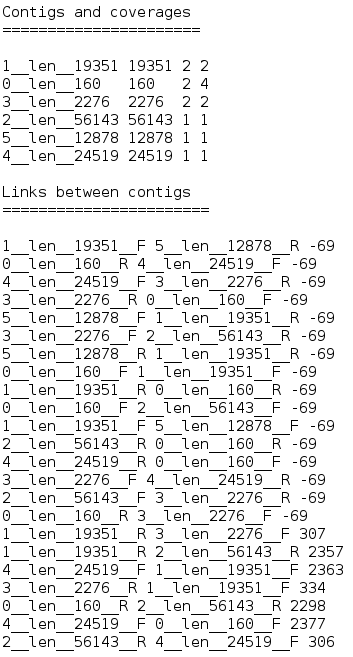
\includegraphics[scale=0.4]{agrostis_INPT_txt}};
\node (graph) at (11.5,0) {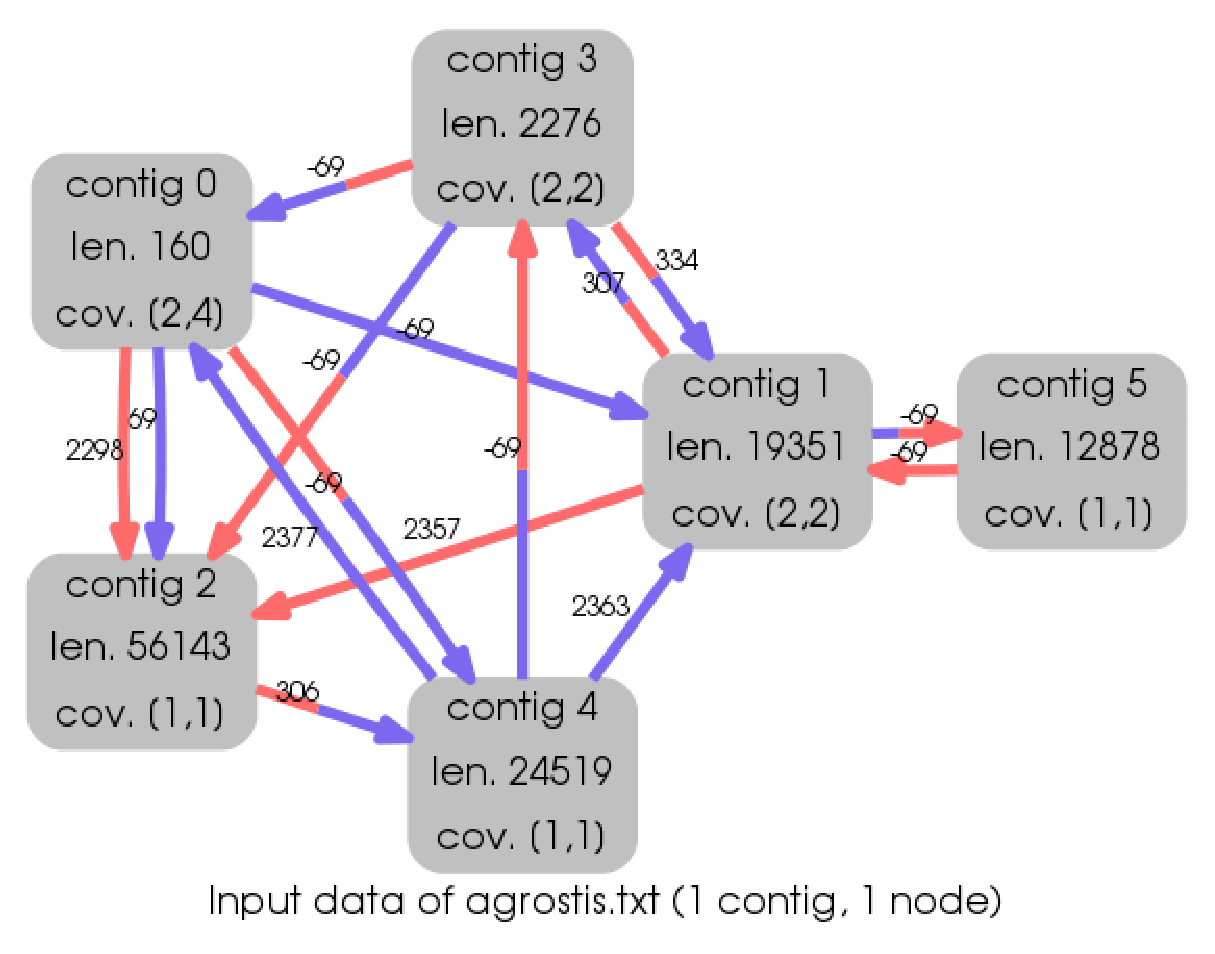
\includegraphics[scale=0.4]{agrostis_INPT_graph}};
\draw [line width=1mm, ->] (txt.east) -- (graph.west) node[midway, above] {\small \texttt{graph\_generator.py}};
\filldraw [color=red] (-2.6,0.4) circle (1.5pt);
\filldraw [color=red] (-2.6,-2.65) circle (1.5pt);
\end{tikzpicture}
}
\caption{Input data of \textit{Agrostis stolonifera} chloroplast genome in \textit{.txt} format and its graph representation}
\label{fig:inpagrostis}
\footnotesize The \textit{.txt} file contains a list of unitigs with their associated length and coverage. When the coverage is $>1$ the unitig is a repeated sequence. The advantage of using unitigs and not contigs is that the associated coverage is easier to determine (for long unitigs) and more trustworthy. For small unitigs, the coverage is an interval (here, the 160bp unitig 0). The joins between unitigs are directed and contain the contig orientation (\textit{Forward} or \textit{Reverse}) information. The distance of each link is negative when two unitigs overlap or positive when two unitigs are separated by a gap. Positive distances (gaps) are obtained though mated-pair information. In the graph, orientations are represented by color: red for \textit{Reverse} and blue for \textit{Forward}.
\end{figure}

\vspace{-0.2cm}
\textbf{How is the \textit{.txt} file obtained? }\\
The data used in this report is artificial. It is simulated from \textit{.fasta} files of reference genomes using two different scripts to generate a paired-end read library and a mated-pair read library. The paired-end read library is used to built unitigs with \textsc{minia} \cite{cascading,minia}, a contig building tool developed at \textsc{Genscale} which supports an unitig building option. The size of the k-mer (minimal number of overlapping bases between two reads for the overlap to be regarded as valid) is chosen so that \textsc{minia} produces the fewest number of unitigs. At this stage published scaffolders can already be used - they require the unitig file and the mated-pair library and perform the read mapping themselves to detect joins. The GST require the mapping process to be separately performed and its input file to roughly resemble the one showed in \ref{fig:inpagrostis}. The GST mapping process has three goals:
\begin{itemize}
\item mapping mated-pairs on large unitigs $\mapsto$ insert size
\item mapping paired reads on unitigs $\mapsto$ unitig coverage
\item mapping mated-pairs on different unitigs $\mapsto$ links between unitigs
\end{itemize}
The bigger the unitig, the more robust the mapping information (homogeneously mapped reads) - hence no exact value for small unitigs' coverage.

\subsubsection{Features of the assembled genomes}
\label{sec:genomefeatures}
As the aim of the Genscale scaffolding project is to produce a complete genome rising to the challenge of repeated sequences. Chloroplastic and bacterial genomes are well suited to test the performances of the GST. Moreover, chloroplastic and bacterial genomes are small enough to enable a fast and detailed assessment and benchmarking of found solutions.

\paragraph*{Chloroplasts}
Chloroplasts are small organelles in plant photosynthetic tissues which possess their own DNA. The chloroplast genomes are small ($\approx 150kpb$), circular and have a large inverted repeated sequence of around $25kpb$. Some instances used in this study lack this repetition. This is the case in \textit{Pinus koraiensis} and \textit{Euglena gracilis}. However these two genomes possess significantly more small ($<$ 20bp) repeated sequences. Figure \ref{fig:chlostructure} shows the classic chloroplastic structure, with colored IR extremities to indicate their relative position, \textit{"facing"} each other in the genome.
\begin{figure}[h!]
\centering
\resizebox{2in}{!}{
\begin{tikzpicture}
   \draw [blue,ultra thick,domain=0:55] plot ({1.6*cos(\x)}, {1.5*sin(\x)});
   \draw [cyan,ultra thick,domain=0:5] plot ({1.6*cos(\x)}, {1.5*sin(\x)});
   \draw [magenta!50,ultra thick,domain=50:55] plot ({1.6*cos(\x)}, {1.5*sin(\x)});
   \draw [red,ultra thick,domain=56:100] plot ({1.6*cos(\x)}, {1.5*sin(\x)});
   \draw [blue, ultra thick, domain=101:160] plot ({1.6*cos(\x)}, {1.5*sin(\x)});
   \draw [magenta!50, ultra thick, domain=101:106] plot ({1.6*cos(\x)}, {1.5*sin(\x)});
   \draw [cyan, ultra thick, domain=155:160] plot ({1.6*cos(\x)}, {1.5*sin(\x)});
   \draw [red, ultra thick, domain=161:359] plot ({1.6*cos(\x)}, {1.5*sin(\x)});
   \node[draw=none, fill=none] at (0,0) {\footnotesize \textsc{Circular genome }};
   \node[draw=none, fill=none] at (0,-0.3) {\footnotesize $\approx 150kpb$};
   \node[draw=none, fill=none] at (1.5,1) {\footnotesize \color{blue} \textbf IR};
   \node[draw=none, fill=none] at (-1.3,1.2) {\footnotesize \color{blue} \textbf IR};
   \node[draw=none, fill=none] at (0,-1.75) {\footnotesize \color{red} \textbf LSC};
   \node[draw=none, fill=none] at (0.5,1.65) {\footnotesize \color{red} \textbf SSC};
\end{tikzpicture}
}
\caption{Chloroplast genome structure}
{\footnotesize Inverted Repeat (IR $ \approx 23kpb$) ; Long Single Copy (LSC); Small Simple Copy (SSC $\approx 85kpb$)}
\label{fig:chlostructure}
\end{figure}

\paragraph*{Bacteria}
Bacterial genomes are bigger ($>$ 1Mbb) and contain many small repeated sequences between 500pb and 1000pb. These genomes have regions which are very hard to assemble because short tandem repeated  sequences won't permit any unitig to be built. Repeats as small as 100bp are detected. 150bp reads covering these regions won't be assembled into any unitig and won't result in any trustworthy join. Regions of the reference genome can be completely absent when reaching the scaffolding step, and it will be made difficult by absent valid join information.
\begin{figure}[h!]
\begin{center}
\resizebox{19cm}{!}{
\begin{tikzpicture}
\node (1000) at (0,0) {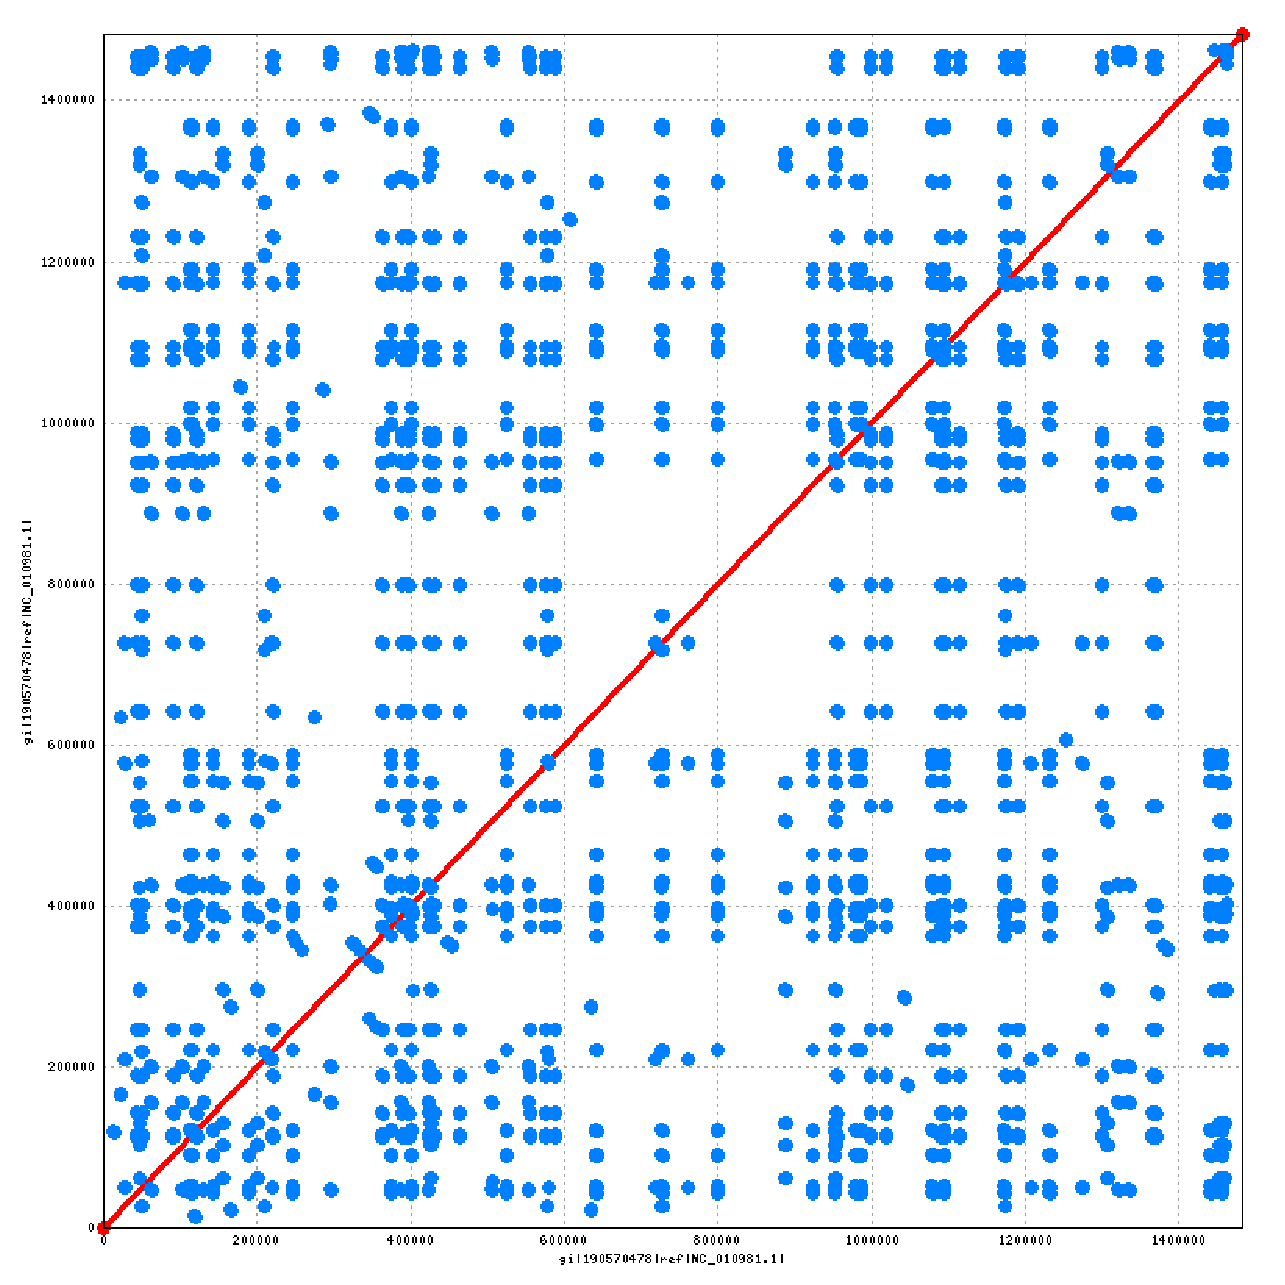
\includegraphics[scale=0.25]{wolba_vs_ref_500}};
\node (500) at (6,0) {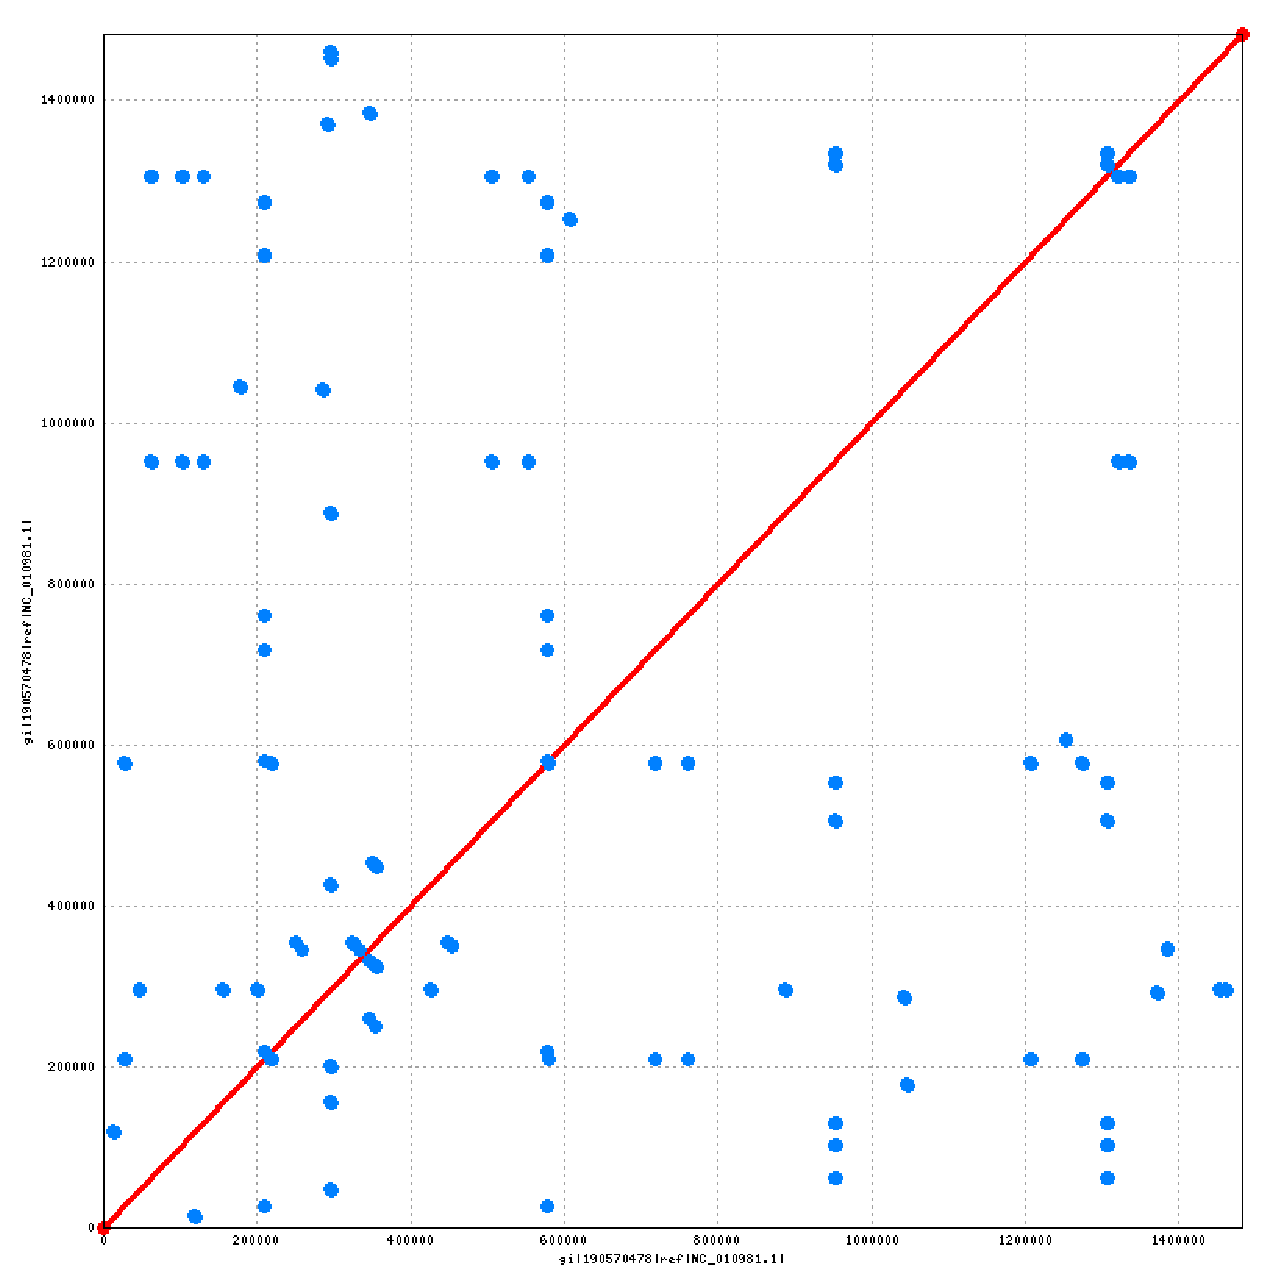
\includegraphics[scale=0.25]{wolba_vs_ref_1000}};
\end{tikzpicture}
}
\end{center}
\caption{\textit{Wolbachia endosymbiont} genome dotplotted against itself}
{\footnotesize The dot-plots were generated by the nucmer script of the MUMmer \cite{delcher_alignment_1999,delcher_fast_2002} sequence fast-alignment tool. (x) and (y) axis are both the \textit{Wolbachia endosymbiont} reference genome downloaded on NCBI 
(\textit{NC\_010981.1}). The blue dots and lines show repetitions in the genome as the DNA sequence matches in several places. The closer the dot is to the red matching axis, the closer the repeats are. We can say, for instance, that at the 1.3Mbp there are several tandem repeats. On the left alignement, repeats longer than 500bp are represented (\texttt{nucmer -l 500} option). On the right repeats longer than 1200bp are represented.}
\label{fig:wolbarepeats}
\end{figure}
\newpage

\subsubsection{Genscale scaffolding problem modeling} \label{sec:gstmodeling}
As seen in figure \ref{fig:inpagrostis}, the input data can be visualized by the \texttt{graph\_generator.py} script as a graph where nodes uniquely represent unitigs regardless of their coverage or orientation. However, this visualization is only useful for a first human assessment of the data. 
Genscale scaffolding tools model each unitig as many times as it occurs. The \texttt{unitig 3} with coverage 2 is transformed into \texttt{unitig 3 occurance 1} and \texttt{unitig 3 occurance 2}, two distinct nodes in the graph. The total number of contig occurrences is then duplicated to model the \textit{Forward} and \textit{Reverse} orientation. \texttt{unitig 3 occurance 1} is transformed into \texttt{unitig 3 occurance 1 \textit{Forward}} and \texttt{contig 3 occurance 1 \textit{Reverse}}. The number of links increases consequently. When transforming joins into model graph links, no duplicate links are allowed (merged) and for each link its reverse equivalent is created. Link coverage is not taken into account. Link weight is the estimated distance between two nodes, which is the space left between the two joined tips of two unitigs. A distance is negative when two unitigs overlap and positive when there is a gap. Gaps are obtained thanks to mated-pair read information: in this case the distance is the estimated length of the pair's insert size minus the remained sequence length of the unitigs following the reads' mapping. A simple example of the difference between the raw input graph and the processed modeled input graph that the GST solve is presented in figure \ref{fig:riceinpt}.

\begin{figure}[h!]
\begin{center}
\resizebox{17cm}{!}{
\begin{tikzpicture}
\node (txt) at (0,0) {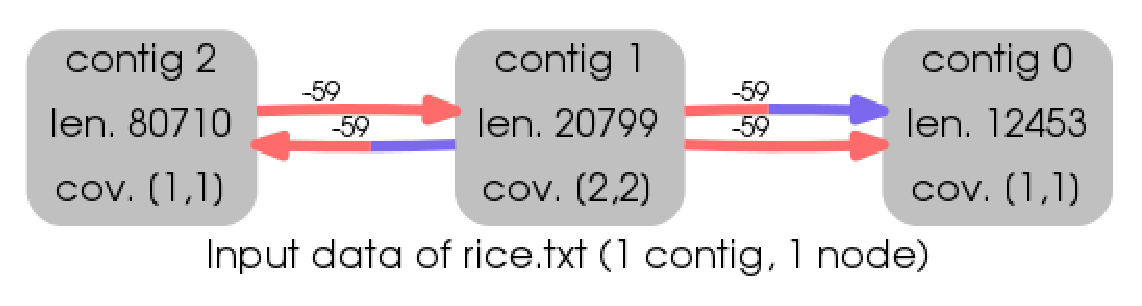
\includegraphics[scale=0.4]{rice_INPT_graph_G1}};
\node (graph) at (11,0) {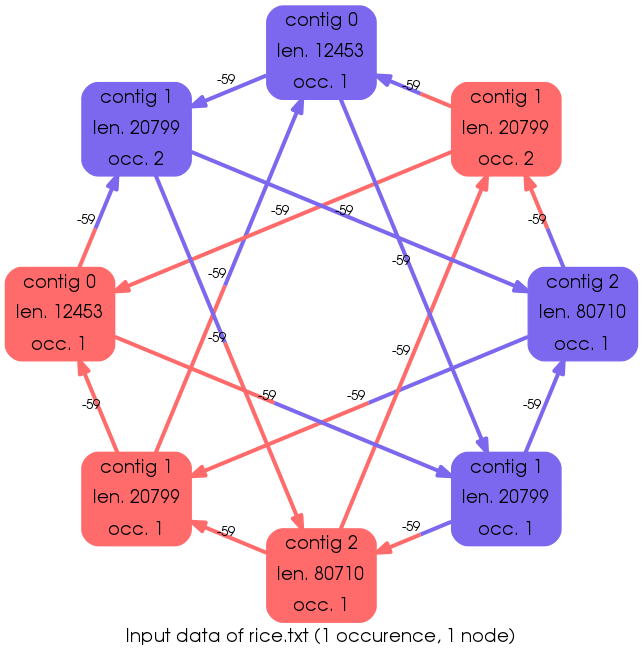
\includegraphics[scale=0.4]{rice_INPT_graph_G2}};
%\draw [line width=1mm, ->] (txt.east) -- (graph.west) node[midway, above] {\small \texttt{graph\_generator.py}};
\end{tikzpicture}
}
\end{center}
\caption{Input graphs of rice, as observed in the \textit{.txt} file (left) and as modeled by the Genscale scaffolding tools (right)}
\footnotesize Sum of unitig occurrences is 4 so the final number of nodes in the model graph is $4\times2=8$. There are no duplicate links in this example. Flipping the model graph (change the link orientation and color and node color) produces all the reverse complement links.
\label{fig:riceinpt}
\end{figure}
\newpage
%-------------------------------------------------------------------------------
% BODEH!
%-------------------------------------------------------------------------------
\subsubsection{Differences between Genscale scaffolding tools}\label{sec:gstdiff}
Although all GST try to solve the problem exactly, different models were developed having different objective functions and input information.
\paragraph*{Weighted path model} Weighted math model (wpm) does not take link weight into account and only aims at solving the order and relative orientation of unitig. The distance between unitig is not known. This model produces several solutions, among them several can be valid or sub-optimal ones. The objective function of this model maximizes the number of links (bundled read pairs) whose orientation corroborates the suggested orientation of unitigs they are linking. All nodes must be visited once because this model doesn't support intervals as unitig coverage. Visually, it means that each node in a solution has $inDegree=outDegree=1$ and $color(inArrow)=color(outArrow)=color(Node)$.

\paragraph*{Distance based model} Distance based model (dist) gives weight to links which is the sequence size between two extremities of two unitigs: negative weight in case of an overlapping and positive weight in case of a mated-pair estimated insert size. It produces a single solution. On an axis from 0 to $\infty$ it tries to find the best position for a unitigs using linear programming so that there are as few as possible erroneous read pairs. The less conflicting data used, the better. The solution provided can contain two consecutive unitigs for which no join exists in the input data if positioning them so helps reducting the number of errors. It doesn't support unitig intervals either but can produce solutions with coverages different from what is provided in the \textit{.txt} files. 


\paragraph*{Flow model} Flow model is currently being developed. The strategy is divided into two steps and relies on the definition of \textit{large unitigs}. This definition evolved in the \textsc{Genscale} team: currently large unitigs are unitigs with a sequence length superior to the biggest mated-pair distance in the input data. The first step of the flow model strategy is to link these large unitigs and construct a genome frame containing gaps. The second step, yet to be implemented, aims at filling in the gaps with the remaining unitigs. This strategy emerged when the wpm was able to construct a genome frame for large datasets (bacterial genomes) once smaller unitigs were filtered out (arbitrary size based filtering). Since then the definition of large contigs evolved and linkage challenges were solved for this first step (see figure \ref{fig:flowlinkage}). Additionally, the flow model supports intervals for contigs coverage and confidence intervals for mated-pair distances.
\iffalse
\begin{algorithm}[h!]
\caption{Flow model Genscale Scaffolding Tool first step algorithm  \\ \footnotesize }
\textbf{begin} \\
compute the highest edge length  $D$ \\
let $N$ be the set of selected nodes\\
let $E$ be the set of selected edges\\
let $H$ be the set of neighbors of a node \\
\textbf{for each} node $n$ : \\
\hspace*{1cm}\textbf{if} $L(n) \leq D $ : \\
\hspace*{2cm}add $n$ to $N$\\
\textbf{for each} node $n$ in $N$: \\
\hspace*{1cm} retrieve $H(n)$ \\
\hspace*{2cm}\textbf{for each} node $h$ in $H$ : \\
\hspace*{3cm}\textbf{if} $h$ in $N$: \\
\hspace*{4cm}add the edge between $n$ and $h$ in $E$: \\

\textbf{end}
\end{algorithm}
\fi

\begin{figure}[h!]
\begin{center}
\resizebox{15cm}{!}{
\begin{tikzpicture}

\node (1F) [draw, text width=2cm, fill=red!30, scale=0.2, align=center] at (0,0) {1 Forward \textsc{large}};
\node (4F) [draw, text width=2cm, fill=red!20!gray, scale=0.2, align=center] at (1,0) {4 Forward \textsc{small}};
\node (3R) [draw, text width=2cm, fill=blue!30, scale=0.2, align=center] at (2,0) {3 Reverse \textsc{large}};
\node (6F) [draw, text width=2cm, fill=red!30, scale=0.2, align=center] at (3,0) {6 Forward \textsc{large}};

\draw[->] (1F.north) to [bend left=55] (4F.north);
\draw[->] (4F.north) to [bend left=55] (3R.north);
\draw[->] (3R.north) to [bend left=55] (6F.north);
\draw[dotted,thin, color=gray] (1F.south) to [bend right=35] (3R.south);

\end{tikzpicture}
}
\end{center}
\caption{Example of a linkage challenge when using solely large unitigs for a genome framework construction}
{\footnotesize If the only way to link unitig 1 to unitig 3 is though unitig 4, and unitig 4 is considered a small one and filtered out for the first step, then the linkage information between unitig 1 and unitig 3 is lost, yet they have to be consecutive in the genome framework. This unitig organization is found in pinus.}
\label{fig:flowlinkage}
\end{figure}


%-------------------------------------------------------------------------------
% BODEH!
%-------------------------------------------------------------------------------
\subsection{Input data features and complexity inspection}
Transforming the input data file into the graph solved by the GST is carried out by the Python interface to the Graphviz \cite{gansner_open_2000,ellson_graphviz_2003} graph layout and visualization package, pygraphviz. Graphviz provides quick methods to access the features of the graph. The Python implementation uses the networkx \cite{hagberg-2008-exploring} package. Features and complexity of the input graph was evaluated with the underlying wish to understand why certain instances were wrongly scaffolded. Automated transformation and inspection of the input data was implemented in the \texttt{graph\_inspector.py} script. Additionally this script can also provide differences between the expected solution and the input data, detecting missing linkage information in the input data.

\subsection{Benchmarking} \label{sec:benchmarking}
Comparing the performance of the GST can be done on several levels. As the data is artificially generated from an already known genome, there is an expected solution. The GST solutions can be compared between themselves, with the expected solution and with solutions provided by other published tools. The solution formats are not the same and automated methods were set up to extract and compare scaffoldings. 

\subsubsection{Comparison with the expected solution}
The expected solution provided by the mapping of unitigs on the reference genome is the one GST aim to obtain in the form of an uninterrupted and accurately gapped scaffold. However in some cases the solution is not unique. In real life several versions of the genome can co-exist, so the GST should aim at providing all valid solutions. In our artificial datasets, only one version of the genome is used, however in the case of chloroplastic genomes the multiple valid solution configuration arises. The Small Single Copy and the Long Single Copy have both extremities next to the same extremities of the two Inverted Repeats (see figure \ref{fig:chlostructure}). In absence of strong mated-pair information overthrowing the overlapping information of these extremities, the SSC and the LSC can be oriented in a \textit{Forward} or a \textit{Reverse} configuration, creating a total of 4 valid combinations. Of course, the genomic structure can be much more complex than that presented in figure \ref{fig:chlostructure}, providing linkage information that would corroborate an orientation over another. The fact is, a valid solution is not an exact copy of the expected solution. Because it is not known in advance which contigs form the IR of the chloroplastic genome and because in \textit{de novo} assembly no assumption of the genomic structure shall be made at all, these alternative solutions are very hard to detect automatically. \\
The detection of exact copies of the expected solution has been implemented in the \texttt{graph\_comparator.py} script. It is a simple list comparison after the retrieval of GST solution in the form of an ordered list of oriented unitigs. Distances between unitigs have been ignored for this comparison. Sub-optimal solutions are also detected. This detection effort has been made especially for the distance based model which provides a single solution sometimes possessing only one or two errors of orientation. However misplacement of a large set of contigs can only be detected visually with the graph provided by the \texttt{graph\_generator.py} script. This kind of error did not occur many times in the instances tested as misplacement of one or several contigs often leads to more errors.

\subsubsection{Comparison with published tools: benchmarking strategy}
A summary of the benchmarking strategy used is presented in figure \ref{fig:benchwork}. Based on the comprehensive evaluation of assembly scaffolding tools \cite{hunt_comprehensive_2014}, the SSPACE scaffolding tool was chosen to be compared to GST. SSPACE is not a graph based scaffolder and its strategy of handling repeats is not explained. For all the other considered scaffolders, it is explicitly written that repeated regions are detected and discarded in order to avoid ambiguous joins. Before proceeding to the benchmarking, solution files from SSPACE and GST were converted. The two converters are :
\begin{itemize}
\item the \texttt{sspace\_2\_order.py} script which takes the SSPACE \textit{.fasta} scaffolding solution and the SSPACE evidence file tracking the scaffold unitig composition, and outputs an ordered list of orientated (possibly extended) unitigs for each scaffold
\item the \texttt{gst\_order\_2\_scaf.py} script which takes the GST solution file and the unitig \textit{.fasta} file and constructs the whole uninterrupted GST scaffold, appending N bases when the distance between unitigs is positive.
\end{itemize}

The \textit{.fasta} files containing the nucleic sequence of scaffolding solution are compared with the Quality Assessment Tool for Genome Assemblies (Quast\cite{gurevich_quast:_2013}). The reference genomes and the gene file downloaded from NCBI are given to Quast for additional metrics.

\texttt{ > quast.py gst\_solution.fasta sspace\_solution.fasta unitigs.fasta \\ -R ref\_genome -G gene\_file.txt -o quast\_output\_dir}

Quast provides 31 metrics with this command, some more pertinent for our study than others. The ones and that will be presented in \fulleref{sec:res} are: 
\begin{itemize}
\item \#scaffolds and \#scaffolds $\geq 1000bp$ : especially interesting to compare it to the \#unitigs
\item total length of scaffolds: detect if any unitig was duplicated (GST) or elongated (SSPACE)
\item largest built scaffold - usually the GST leads to one single large scaffold
\item N50:  length for which the collection of all contigs of that length or longer covers at least 50\% of assembly length. Extensively used metric, but considering the GST solution aims at large unique solution, this metric is a nice indication for SSPACE. It is also useful for the \textsc{gensclae} flow model, which is not finished yet and produces several disconnected scaffolds.
\item \#misassemblies, \#mismatches and \#indels
\item genome fraction assembled 
\item Ns per 100kbp: Ns are added in SSPACE scaffolds, flow and distance based model
\item \#genes found
\item largest accurate alignment with the reference genome
\end{itemize}
A visualization of the solution is necessary as Quast does not provide information on ordering of unitigs. The presence of misassemblies is an indication of a possible order mistake however it can also be small distance between unitigs errors resulting in wrong overlapping or extra Ns. A visual alignment of the scaffolding sequences with the reference genome is a sturdy method to evaluate the scaffolding continuity. Dotplots are generated with \texttt{nucmer}, of the MUMmer software. Two steps are necessary: 
\begin{itemize}
\item \texttt{nucmer scaffolding.fasta ref\_genome.fasta -l 500} aligns the two nucleic sequences and outputs a \textit{.delta} file. The \texttt{-l} option registers all alignements which are superior to 500bp.
\item \texttt{mummerplot nucmer\_output.delta -t png} outputs a dotplot in \textit{.png} format.
\end{itemize}
The MUMmer software also provides the \texttt{show-coords} tool which detects and outputs the list of coordinates of selected regions of the alignement. For example:
\begin{itemize}
\item \texttt{show-coords -l -T -L 1200 -q nucmer\_alignement.delta} outputs a tab delimited file (\texttt{-T}) containing alignements longer than 1200bp (\texttt{-L}), including the sequence length (\texttt{-l}).
\end{itemize}
Sequence continuity is evaluated thanks to this methodology, it does not however show the unitigs that board the eventual misassemblies or continuity rupture. Unscaffolded unitigs and wrongly scaffolded unitigs are detected with \texttt{graph\_constructor.py}. Their environment in the input data is analyzed in order to understand the reason behind the scaffolding failure.

\begin{figure}[h!]
\begin{center}
\resizebox{16cm}{!}{
\begin{tikzpicture}
\node[text width=5cm,align=left] (filetit) [draw=none] at (0.5,0.6) {\textsc{\tiny (1) file format standardisation}};
\draw[fill=gray!5] (-2.3,0.5) -- (3.4,0.5) -- (3.4,-5) -- (-2.3,-5) -- (-2.3,0.5);
\node[text width=3cm,align=center] (mp) [draw, fill=blue!20, scale=0.5] at (0,0) {\textsc{mate pairs}};
\node[text width=2cm,align=center] (unitigs) [draw, fill=red!20, scale=0.5] at (2,0) {\textsc{unitigs}};

\node (arrowbase) [draw=none, shape=circle, fill=black, scale=0.15] at (1,-1) {};

\node[text width=3cm,align=center] (scaf) [draw, fill=green!20, scale=0.5] at (0,-2) {\textsc{sspace scaffolds}};
\node[text width=3cm,align=center] (list) [draw, fill=magenta!20, scale=0.5] at (2,-2) {\textsc{gst ordered unitigs}};

\draw (unitigs.south) to [bend left=35] (arrowbase.north);
\draw (mp.south) to [bend left=-35] (arrowbase.north);

\draw[->] (arrowbase.south) to [bend left=20] (scaf.north);
\draw[->] (arrowbase.south) to [bend right=20] (list.north);

\node[scale=0.3] (scafsspace) at (0, -1.35) {\textit{SSPACE\_Standard\_v3.0.pl}} ;
\node[scale=0.3] (scafgst) at (1.8, -1.35) {\textit{genscale\_scaf.py}} ;

\node[text width=3cm,align=center] (list2) [draw, fill=magenta!20, scale=0.5] at (0,-4) {\textsc{\small sspace ordered contigs}};
\node[text width=3cm,align=center] (scaf2) [draw, fill=green!20, scale=0.5] at (2,-4) {\textsc{gst scaffolds}};

\draw [->] (scaf.south) -- node[scale=0.7, left] {\tiny \textit{sspace\_2\_order.py}} (list2.north);
\draw [->] (list.south) -- node[scale=0.7, right] {\tiny \textit{gst\_order\_2\_scaf.py}} (scaf2.north);

\node[text width=2cm,align=center] (evidence) [draw, fill=cyan!20, scale=0.3] at (0.9,-2.6) {\textsc{sspace evidence file}};
\draw (evidence.west) to [bend right=23] (list2);

\node[text width=2cm,align=center] (unitigsbis) [draw, fill=red!20, scale=0.3] at (1.5,-3) {\textsc{unitigs}};
\draw (unitigsbis.east) to [bend left=10] (scaf2);

%somearrows
\node (A) [draw=none, shape=circle] at (-1.7,0.5) {};
\node (B) [draw=none, shape=circle] at (-1.7,-2.1) {};
\node (C) [draw=none, shape=circle] at (-1.7,-5) {};

\draw[sloped, anchor=center, above, text width=2.0cm, thick, dotted] (B) -- node{\tiny \textsc{scaffolding}} (A);


\draw[sloped, anchor=center, above, text width=2.0cm,thick, dotted] (C) -- node{\tiny \textsc{data parsing}}(B);

%benchmarking titles
\node[text width=3cm,align=left] (quasttit) [draw=none] at (5.5,0.6) {\textsc{\tiny (2) quast benchmarking}};
\node[text width=3cm,align=left] (hometit) [draw=none] at (5.5,-2.9) {\textsc{\tiny (3) home benchmarking}};
\draw[fill=green!5] (3.5,0.5) -- (7,0.5) -- (7,-2.5) -- (3.5,-2.5) -- (3.5,0.5);
\draw[fill=magenta!5] (3.5,-3) -- (7,-3) -- (7,-5) -- (3.5,-5) -- (3.5,-3);
%benchmarking quast guts
\node[text width=2cm,align=center] (scafs) [draw, fill=green!20, scale=0.5] at (4.2,0.2) {\textsc{scaffolds}};
\node[text width=2cm,align=center] (unitigs) [draw, fill=red!20, scale=0.5] at (4.2,-0.3) {\textsc{unitigs}};
\node[text width=3cm,align=center] (refgenome) [draw, fill=gray!20, scale=0.5] at (6,0.2) {\textsc{ref. genome}};
\node[text width=3cm,align=center] (gfile) [draw, fill=gray!20, scale=0.5] at (6,-0.3) {\textsc{gene file}};
\node[text width=1cm, align=center] (quastbam) [draw, thick, fill=green!45] at (5,-1.2) {\textsc{\tiny quast}};
\draw[thin, ->] (scafs.east) to [bend left=10] (quastbam.north);
\draw[thin, ->] (refgenome.west) to [bend left=-10] (quastbam.north);
\draw[thin] (unitigs.east) to [bend left=10] (quastbam.north);
\draw[thin] (gfile.west) to [bend left=-10] (quastbam.north);
\node[text width=4cm, align=center] (metrics) [draw, fill=white, scale=0.5] at (5.4,-2) {\textsc{assembly quality metics comparison}};
\draw[thin, ->] (quastbam.west) to [bend left=-75] (metrics.west);
%benchmarking home guts
\node[text width=6cm,align=center] (orders) [draw, fill=magenta!20, scale=0.5] at (5.2,-3.2) {\textsc{\scriptsize ordered lists of oriented contigs}};
\node[text width=2.5cm,align=center] (mummer) [draw, thick, fill=magenta!40, scale=0.5] at (4.3,-3.8) {\textsc{nucmer}};
\node[text width=3.2cm,align=center] (constructor) [draw, thick, fill=magenta!40, scale=0.45] at (6,-3.8) {\textit{\footnotesize graph\_constructor.py}};

\draw[thin, ->] (orders.south) to [bend left=-20] (mummer.north);
\draw[thin, ->] (orders.south) to [bend left=20] (constructor.north);

\node[text width=5cm,align=center] (viz) [draw, fill=white, scale=0.45] at (5.2,-4.7) {\textsc{visual assessment of scaffolding quality}};

\draw [->] (mummer.south) -- node[scale=0.7, left] {\tiny \textit{dotplots}} (viz.north);
\draw [->] (constructor.south) -- node[scale=0.7, right] {\tiny \textit{graphs}} (viz.north);
\end{tikzpicture}
}
\end{center}
\caption{Benchmarking workflow}
\label{fig:benchwork}
\footnotesize (1) SSPACE provides a \textit{.fasta} file with built scaffolds. The \texttt{sspace\_2\_order.py} script converts it to the GST solution format. The GST do not compute \textit{.fasta} sequences of unitigs. The scaffolding final result is an ordered list of unitigs. The \texttt{gst\_order\_2\_scaf.py} script converts the solution to a \textit{.fasta} format. If distances between unitigs are not available, the k-mer size with which the unitigs were built is used. \\
\footnotesize (2) The reference genome and gene file provide additional metrics for assembly comparison with Quast (number of found genes, percentage of genome assembled, N50 \ldots). All files in \textit{.fasta} format are compared with Quast. \\
\footnotesize (3) Further inspection of scaffolding solutions is done thanks to \texttt{nucmer} alignment tool. \texttt{nucmer} dotplots scaffolding solutions against the reference genome so challenging regions can be detected. The \texttt{graph\_constructor.py} aids the detection of unitigs which were wrongly assembled.
\end{figure}

%-------------------------------------------------------------------------------
% BODEH!
%-------------------------------------------------------------------------------
\clearpage
\section{Results}\label{sec:res}
\subsection{Comparison between the data sets}
Results presented in table \ref{tab:graphcomplexity} are obtained with the \texttt{graph\_inspector.py} script. The analysed graph is the one modeled by the GST and built by the \texttt{graph\_generator.py} script (see rice example figure \ref{fig:riceinpt}). 

\begin{table}[h!]
\resizebox{18cm}{!}{
\begin{tabular}{|l||c|c|c|c|c|c|c|c|c|c||r|}
\hline
organism & G type & G size (bp) & \#nodes & \#edges & node degree & graph density & diameter & \#periphery n. & radius & \#central n. & status\\  
\hline
agrostis & chpl. &136584& 22 & 98 & min  4 , max  13 , avg  8 & 0.212 &6 & 1 & 4 & 6 & solved\\
acineto & bacter &3598621& 924 & 7984 & min  0 , max  114 , avg  17 & 0.009 &gnc:ipl&gnc:ipl&gnc:ipl& gnc:ipl& unsolved\\
acorus & chpl.&153821& 30 & 204 & min  4 , max  26 , avg  13 & 0.234 &5 & 13 & 4 & 17& solved \\
atropa & chpl.&156687& 52 & 268 & min  5 , max  16 , avg  10 & 0.101 &8 & 12 & 6 & 6& solved\\
cucumis & chpl.&155293& 194 & 1446 & min  4 , max  50 , avg  14 & 0.038 &11 & 30 & 8 & 6& solved\\
eucalyptus & chpl.&160286& 8 & 16 & min  4 , max  4 , avg  4 & 0.285 &4 & 8 & 4 & 8& solved\\
euglena & chpl.&143171& 296 & 11894 & min  12 , max  176 , avg  80 & 0.136 & gnc:ipl&gnc:ipl & gnc:ipl&gnc:ipl& unsolved \\
lecomtella & chpl.&139073& 22 & 90 & min  4 , max  13 , avg  8 & 0.194 &6 & 3 & 4 & 5& solved\\
oenothera & chpl.&163935& 172 & 3086 & min  4 , max  70 , avg  35 & 0.104 &14 & 1 & 9 & 47& solved\\
pinus & chpl.&116866& 122 & 628 & min  4 , max  29 , avg  10 & 0.042 &13 & 7 & 7 & 1& almost solved\\
rice & chpl.&134525& 8 & 16 & min  4 , max  4 , avg  4 & 0.285 &4 & 8 & 4 & 8& solved\\
sacchar. & chr3 &316613& 370 & 4416 & min  4 , max  113 , avg  23 & 0.032 &13 & 1 & 6 & 37& unsolved\\
wolbachia & bacter &1482355& 4270 & 616804 & min  5 , max  2582 , avg  288 & 0.033 & 9 & 23 & 5 & 198& unsolved\\
\hline
\end{tabular}
}
\caption{GST modeled graph features}
\footnotesize \textit{\color{magenta}G.}: genome, \textit{\color{magenta}n.}: nodes, \textit{\color{magenta}chpl.}: chloroplast, \textit{\color{magenta}bacter.}:bacterial, \textit{\color{magenta}chr3}: chromosome 3, \textit{\color{magenta}gnc:ipl}: "graph not connected: infinite path length".\\
{\color{magenta} node degree}: the number of edges incident to the vertex. Self-loops are not allowed in this graph.\\
{\color{magenta} graph density}: $D(G)=\frac{\lvert L \lvert}{\lvert N \lvert(\lvert N \lvert-1)}$ with $\lvert L \lvert$ the link cardinal and $\lvert N \lvert$ the node cardinal. A dense graph has a  number of links close to the maximal number of link, and a density value close to $1$. \\
{\color{magenta} graph diameter}: greatest geodesic distance (shortest path between two nodes) for any node in the graph. \\
{\color{magenta} graph periphery}: nodes with maximal eccentricity (geodesic distance $=$ diameter).\\
{\color{magenta} graph radius}: lowest geodesic distance for any node in the graph.\\
{\color{magenta} graph center}: nodes with minimal eccentricity (geodesic distance $=$ radius).\\
\label{tab:graphcomplexity}
\end{table}

The minimal degree for a node in the graphs should be 4 because a node has at least an in-going link and an outgoing link ($indegree=outdegree=1$). The graph also models their reverse equivalents. Acineto has a node degree equal to 0. It means an unitig is completly disconnected from the rest of the genome. This explains the "graph not connected" error and why it is unsolvable. Furthermore the density of the graph is very low. Euglena however has a minimum node degree of 12. There are no nodes with indegree or outdegree equal to 0. This could indicate that the euglena graph holds two disconnected sub-graphs. \\
The two smallest graphs have the highest graph density: the graphs have 8 nodes with $indegree=outdegree=1$, ($\times 2$ because of the reverse equivalent links). All links are overlaps. All degrees are all equal to 4. Lower densities indicate that not all consecutive unitigs have joins between them and their consecutive ordering need to be deduced from mated-pair information with other non consecutive unitigs. The three solved instances with the most nodes (cucumis, oenothera and pinus) have low graph density and also have the highest diameter and radius. Distance between nodes are big. Graph periphery in these instances contains mainly short repeat nodes which lack mated-pairs. These nodes are poorly connected to the rest of the graph despite the need for them to be used multiple times.

At the beginning of the project the idea of detecting inconsistencies in the input data by comparing input links with the expected solution links was tested. These results are presented for the chloroplastic instances in table \ref{tab:compgsi}. Links in the input solution are links between consecutive unitigs (no mated-pair reads obviously). The high number of links in the input absent from the expected solution comes from the fact that mated-pairs usually link non consecutive unitigs. This strategy has  lead to some explanations for GST' difficulties in scaffolding pinus. A link in the expected solution (link between two consecutive unitigs) was absent in the input data. As previously seen, consecutive unitigs are not always joined in the input data. However in pinus, the unitigs 14 and 15 were linked in the \texttt{14 Forward -> 15 Reverse} order when the expected order was \texttt{14 Reverse -> 15 Forward} (these two links are not reverse equivalent). This lead to a wrong graph model. The pinus data was eventually re-simulated and solved with the flow model. 

\begin{table}[h!]
\centering
\resizebox{7cm}{!}{
\begin{tabular}{|l||c| c|}
\hline
organism & links in I and not in ES & links in ES and not in I \\
\hline
eugalyptus & 0 ($0\%$) & 0 \\
atropa & 6 ($42.8\%$) & 0 \\
lecomtella & 11 ($64.7\%$) & 0 \\
oenothera & 18 ($43.9\%$) & 0 \\
cucumis & 79 ($69.9\%$) & 0 \\
pinus & 23 ($60.5\%$)& 2 \\
euglena & 79 ($73.1\%$) & 0 \\
\hline
\end{tabular}
}
\caption{Comparison between the input linking data and the expected solution's links}
\footnotesize {\color{magenta}I}:input data, {\color{magenta}ES}:expected solution
\label{tab:compgsi}
\end{table}



\subsection{Comparison of GST solutions with the expected solution}

Valid solutions were detected with the \texttt{graph\_comparator.py} script. Other sub-optimal solutions were looked for manually. The GST performance are presented in table \ref{tab:solutions}. 

\begin{table}[h!]
\begin{center}
\resizebox{18cm}{!}{
\begin{tabular}{|l||c|c||c|c||l|}
\hline
organism & expected solution found & time & partial solution found & time & note\\
\hline
agrostis &wpm&0.5s&-&-&1 valid solution among 4, sub-optimal found with dist and flow \\
acineto &-&-&wpm&0.6s& ordering big unitigs correctly \\
acorus &wpm&0.5s&-&-&1 valid solution among 2, also found with dist and flow \\
atropa &wpm&1s&-&-&1 valid solution among 2, also found with flow \\
cucumis &wpm&35s&-&-&several valid solution among 18 \\
eucalyptus &wpm&0.2s&-&-&1 valid solution among 2, also found with dist and flow \\
euglena &-&-&-&-& instance never fully or partially solved \\
lecomtella &wpm&0.6s&-&-&1 valid solution among 4, sub-optimal found with dist \\
oenothera &wpm&163s&-&-&1 valid solution among 4 \\
pinus &-&-&flow&0.2&instance never solved with wpm or dist, good frame found with flow \\
rice &flow&0.1s&-&-&also found with wpm and dist \\
sacchar. &-&-&-&-&instance never fully or partially solved \\
wolbachia &-&-&flow&0.4s& built frame with large unitigs resulting in 11 disconnected scaffolds \\
\hline
\end{tabular}
}
\end{center}
\caption{Genscale scaffolders solutions}
\label{tab:solutions}
\end{table}

Pinus and euglena are the two chloroplastic genomes which were not fully solved by first generation GST tools. They are incidentally the two chloroplasts not to possess an inverted repeat. Pinus has a significantly shorter genomic length. As noticeable in table \ref{tab:graphcomplexity}, the number of nodes is not linked to the genome size but rather to the amount of repeated sequences assembled into separate unitigs. Pinus is partially solved by the first step of the flow model (92.1\% of the genome assembled). Bacterial genomes are very challenging to scaffolds for reasons described in section \fulleref{sec:genomefeatures}. Building a genomic framework is now possible with the flow model, but the full genome has yet to be scaffolded. Results for wolbachia are further discussed in section \fulleref{sec:wolbachia}. \\
\centerline { $ * \quad * \quad * $ }
\vspace{0.5cm}

Next sections present results obtained with the benchmarking workflow. Promising results are detailed using the agrostis example, but the excellent performance of GST for agrostis is also valid for other chloropastic genomes (except pinus and euglena). The improvement in scaffolding made with the flow model will be detailed for pinus. But one must keep in mind that for now only the first frame building step of the flow model was benchmarked, consequently the fraction of the assembled genome will often be quite low.

\newpage
\subsection{Comparison of the best GST solutions and SSPACE to the reference genome}
As a reminder, the reason why SSPACE was chosen is because it performs very well according to the comparative scaffolding study \cite{hunt_comprehensive_2014-1} and it does not explicitly discard repetitive regions.
\subsubsection{Quality assessment of genome assemblies of \textit{Agrostis stolonifera} chloroplastic genome}

\paragraph*{QUAST} 
\textit{Agrostis stolonifera}  chloroplastic genome was successfully assembled with the Weighted path model. The wpm provides 4 solution, among them two are valid ones ($1^{st}$ and $2^{nd}$) and one ($1^{st}$) is the exact copy of the expected solution (the reference genome). The wpm scaffold solution was rebuilt using the size of the k-mer used during the unitig building step (60bp) in place of unitig distance information. Each unitig overlaps its unitig neighbors for 59bp. This method leads to an exact built solution (100\% of the genome is assembled, same size as the reference). The distance solution is also a satisfying solution however the sizes of the distances between contigs are false and cause the scaffold to be wrongly gapped. The added Ns in the found false gaps increases the size of the genome by 561bp. This is a negligible amount and is not detected by the \textit{N's per 100kpb} metric. The largest alignment is quite low for the distance based model (102364bp before making a misassembly). This length comprises the LSC and an IR, meaning that distance based fails to find the correct distance between the SSC and the IRs. \\ All of the GSTs perform better than the SSPACE scaffolder. Among the 6 unitigs of the agrostis input data, SSPACE does not scaffold the small 160bp unitig and the big 12928bp extended unitig. The three SSPACE scaffolds are:
\begin{itemize}
\item the 160bp contig (0) which is part of the IR ($IR=c3+c0+c1$)
\item the LSC ($LSC=c4+c0+c2$) and an incomplete IR copy lacking the 160bp contig
\item the SSC ($SSC=c5$)
\end{itemize}
The 160bp contig and the SSC possess conflicting links, and SSPACE is not able to take a decision so it does not take the risk of scaffolding them. It does not find the whole genome: only 84.5\% is assembled, which is a 0.3\% more than the sum of all unitig sizes. This slight increase occurs because the extension though unused reads was permitted ($-x=1$ option). However SSPACE can not go much beyond this percentage as it does not compute unitig coverage and is not meant to duplicate any given sequence. 

%AGROSTIS TABLE DAWG
\begin{table}[h!]
\begin{center}
\resizebox{15.5cm}{!}{
\begin{tabular}{|l*{8}{|r}|}
\hline
Assembly & unitigs & wpm\_sol1.fsa & wpm\_sol2.fsa & wpm\_sol3.fsa & wpm\_sol4.fsa & dist\_sol & sspace\_sol & ref\_genome \\ \hline
\# scaffolds ($\geq$ 0 bp) & 6 & {\bf 1} & {\bf 1} & {\bf 1} & {\bf 1} &{\bf 1} & 3 & {\bf 1} \\ \hline
\# scaffolds  ($\geq$ 1000 bp) & 5 & {\bf 1} & {\bf 1} & {\bf 1} & {\bf 1} & {\bf 1} & 2 & {\bf 1} \\ \hline
Total length ($\geq$ 0 bp) & 115327 & 136584 & 136584 & 136584 & 136584 & {\bf 137145} & 115344 & 136584 \\ \hline
Total length ($\geq$ 1000 bp) & 115167 & 136584 & 136584 & 136584 & 136584 & {\bf 137145} & 115184 & 136584 \\ \hline
\# scaffolds  & 5 & {\bf 1} & {\bf 1} & {\bf 1} & {\bf 1} & {\bf 1} & 2 & {\bf 1} \\ \hline
Largest scaffolds  & 56143 & 136584 & 136584 & 136584 & 136584 & {\bf 137145} & 102256 & 136584 \\ \hline
Total length & 115167 & 136584 & 136584 & 136584 & 136584 & {\bf 137145} & 115184 & 136584 \\ \hline
Reference length & 136584 & 136584 & 136584 & 136584 & 136584 & 136584 & 136584 & 136584 \\ \hline
GC (\%) & 37.39 & 38.45 & 38.45 & 38.45 & 38.45 & 38.45 & 37.40 & 38.45 \\ \hline
Reference GC (\%) & 38.45 & 38.45 & 38.45 & 38.45 & 38.45 & 38.45 & 38.45 & 38.45 \\ \hline
\# misassemblies & {\bf 0} & {\bf 0} & 2 & 1 & 1 & 2 & 1 & {\bf 0} \\ \hline
\# misassembled scaffolds  & {\bf 0} & {\bf 0} & 1 & 1 & 1 & 1 & 1 & {\bf 0} \\ \hline
Misassembled scaffolds length & {\bf 0} & {\bf 0} & 136584 & 136584 & 136584 & 137145 & 102256 & {\bf 0} \\ \hline
\# local misassemblies & {\bf 0} & {\bf 0} & {\bf 0} & {\bf 0} & {\bf 0} & 1 & {\bf 0} & {\bf 0} \\ \hline
\# unaligned scaffolds  & 0 + 0 part & 0 + 0 part & 0 + 0 part & 0 + 0 part & 0 + 0 part & 0 + 0 part & 0 + 0 part & 0 + 0 part \\ \hline
Unaligned length & 0 & 0 & 0 & 0 & 0 & 0 & 0 & 0 \\ \hline
Genome fraction (\%) & 84.219 & {\bf 100.000} & {\bf 100.000} & 98.657 & 98.657 & 91.522 & 84.590 & {\bf 100.000} \\ \hline
Duplication ratio & 1.001 & 1.000 & 1.155 & 1.014 & 1.014 & 1.097 & {\bf 0.997} & 1.000 \\ \hline
\# N's per 100 kbp & {\bf 0.00} & {\bf 0.00} & {\bf 0.00} & {\bf 0.00} & {\bf 0.00} & 218.75 & 12.15 & {\bf 0.00} \\ \hline
\# mismatches per 100 kbp & 0.00 & 0.00 & 0.00 & 0.00 & 0.00 & 0.00 & 0.00 & 0.00 \\ \hline
\# indels per 100 kbp & {\bf 0.00} & {\bf 0.00} & {\bf 0.00} & {\bf 0.00} & {\bf 0.00} & 5.60 & 0.87 & {\bf 0.00} \\ \hline
\# genes & 110 + 4 part & 132 + 1 part & {\bf 133 + 0 part} & 131 + 0 part & 131 + 0 part & 122 + 1 part & 114 + 2 part & {\bf 133 + 0 part} \\ \hline
Largest alignment & 56143 & {\bf 136584} & 81612 & 82913 & 134750 & 102364 & 81140 & {\bf 136584} \\ \hline
NA50 & 24519 & {\bf 136584} & 81612 & 82913 & 134750 & 102364 & 81140 & {\bf 136584} \\ \hline
\end{tabular}
}
\end{center}
\footnotesize All statistics are based on contigs of size $\geq$ 50 bp. {\color{magenta}wpm}: weighted path model, {\color{magenta}dist}: distance based model.
\caption{QUAST metrics for the unitig set and several scaffolding solutions of \textit{Agrostis stolonifera} with GST (wpm and dist) and SSPACE}
\label{tab:agro}
\end{table}

\paragraph*{graph\_generator.py}
Figure \ref{fig:scafsols} is a \texttt{graph\_generator.py} visualization of scaffolding solutions compared with Quast in table \ref{tab:agro}. The circled or lined unitigs are those forming the IR of agrostis. This technique visually confirms that the unitigs that SSPACE found challenging to scaffold are the repeated ones. The difference between the two valid solutions found by wpm is also highlighted. The LSC (\textit{c2-c4-c4}) region is reversed but the SSC (\textit{c5}) has the same orientation in both solutions. 

\begin{figure}[h!]
\begin{center}
\resizebox{18cm}{!}{
\begin{tikzpicture}
\node (wpm1) at (0,0) {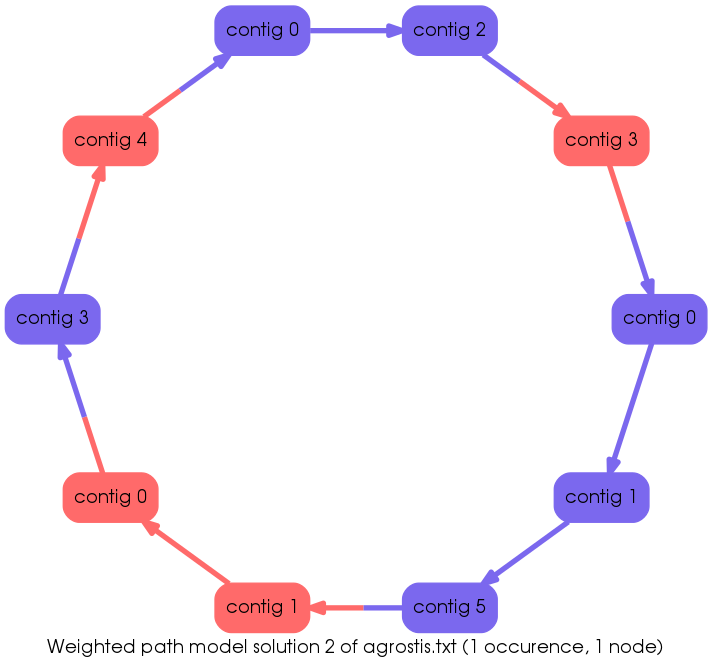
\includegraphics[scale=0.25]{wpm_agrostis_sol1}};
\node (wmp2) at (8,0) {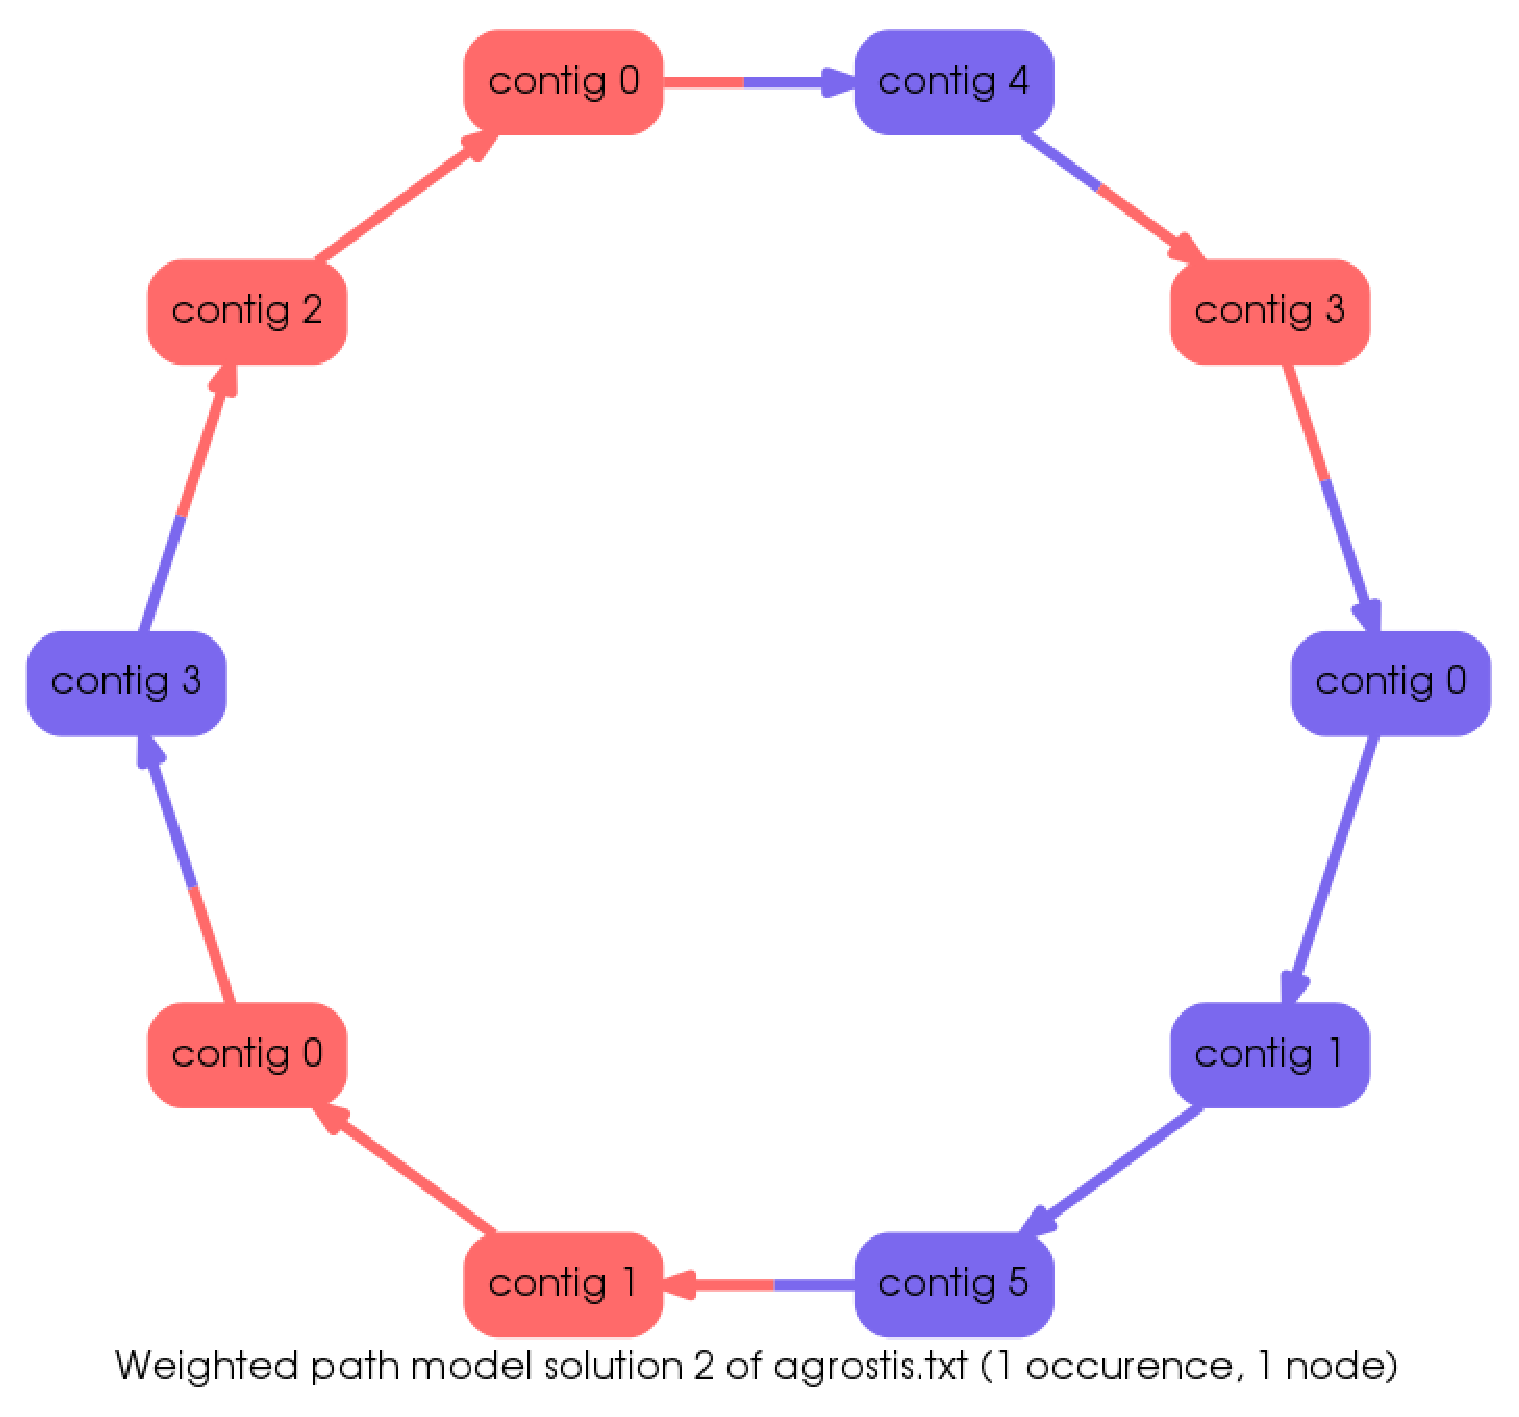
\includegraphics[scale=0.25]{wpm_agrosti_sol2}};
\node (sspace) at (9,7) {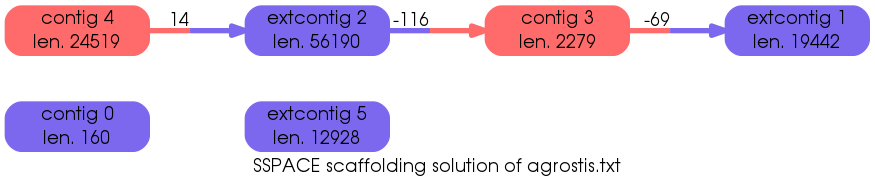
\includegraphics[scale=0.25]{sspace_scaffolds_agrostis}};
\node (gold) at (0,7) {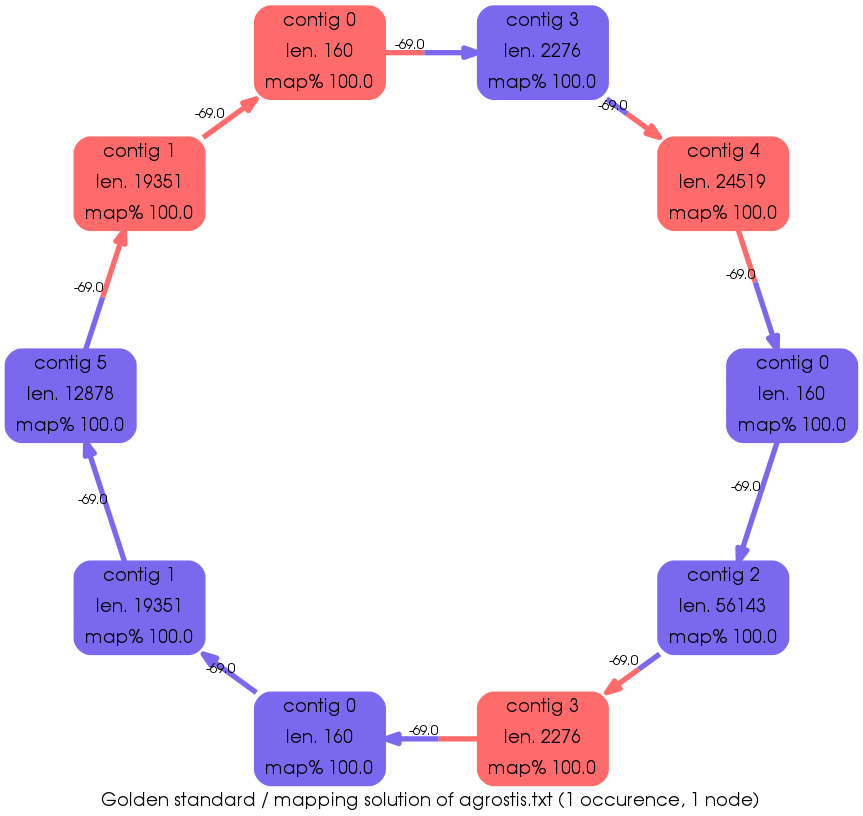
\includegraphics[scale=0.25]{agrostis_GOLD}};

\draw [blue!30,ultra thick,domain=-30:40] plot ({3.3*cos(\x)}, {3.3*sin(\x)});
\draw [blue!30,ultra thick,domain=175:235] plot ({3.3*cos(\x)}, {3.3*sin(\x)});
\draw [blue!30,ultra thick,domain=240:255] plot ({3.3*cos(\x)}, {3.3*sin(\x)});
\begin{scope}[shift={(8,0)}]
\draw [blue!30,ultra thick,domain=-30:40] plot ({3.3*cos(\x)}, {3.3*sin(\x)});
\draw [blue!30,ultra thick,domain=175:235] plot ({3.3*cos(\x)}, {3.3*sin(\x)});
\draw [blue!30,ultra thick,domain=240:255] plot ({3.3*cos(\x)}, {3.3*sin(\x)});
\end{scope}
\begin{scope}[shift={(0,7.1)}]
\draw [blue!30,ultra thick,domain=70:150] plot ({3.9*cos(\x)}, {3.9*sin(\x)});
\draw [blue!30,ultra thick,domain=210:245] plot ({3.9*cos(\x)}, {3.9*sin(\x)});
\draw [blue!30,ultra thick,domain=250:290] plot ({3.9*cos(\x)}, {3.9*sin(\x)});
\end{scope}
\begin{scope}[shift={(11,7.5)}]
\draw [blue!30,ultra thick,domain=0:360] plot ({2*cos(\x)}, {1*sin(\x)});
\end{scope}
\begin{scope}[shift={(5.9,6.7)}]
\draw [blue!30,ultra thick,domain=0:360] plot ({1*cos(\x)}, {0.5*sin(\x)});
\end{scope}

\end{tikzpicture}
}
\end{center}
\caption{Expected solution and scaffolding solutions of the weighted-path model and SSPACE scaffolders}
\footnotesize The expected solution graph (top left) has the contigs correctly ordered, displays their length and their mapping score. The expected solution is obtained by mapping unitigs on the reference genome. The two bottom graphs are two valid wpm solutions and the top right graph is the SSPACE scaffolder solution. \\ \texttt{> graph\_constructor.py -g [expt,whpm,sspace] -f solution\_file.txt}

\label{fig:scafsols}
\end{figure}

\paragraph*{MUMer}
The dotplots further illustrate the differences between the scaffolding solutions. Dotplots do not visualize unitigs but rather the whole scaffolding sequence. If the sequence on the $x$ axis matches the sequence of the $y$ axis in the "$right$" order (both same orientation), a red matching line is drawn. For the control dotplot, where the reference genome is dotplotted against itself a perfect match can be seen. Additionally the inverted repeats are seen as an additional match in the "$wrong$" order (as they are inverted and the orientation is different) and appear as blue lines - little inverted regions are detected. The control dotplot and the first solution of the wpm display the exact same dotplot profile (just shifted, as the \textit{.fasta} files do not start at the same genomic position). In the second solution, a reversed match exists but the small single copy is reversed between the two IRs: the reverse match is interrupted. \\ The SSPACE solution has three scaffolds (3 scaffold names on the side of the graph) and only one occurrence of the IR. Additionally the LSC and IR are scaffolder in the wrong relative orientation which indicates the coordinate of the misassembly detected by Quast (around the 81000bp).

\begin{figure}[h!]
\begin{center}
\resizebox{17cm}{!}{
\begin{tikzpicture}
\node (wpm1) at (0,-7) {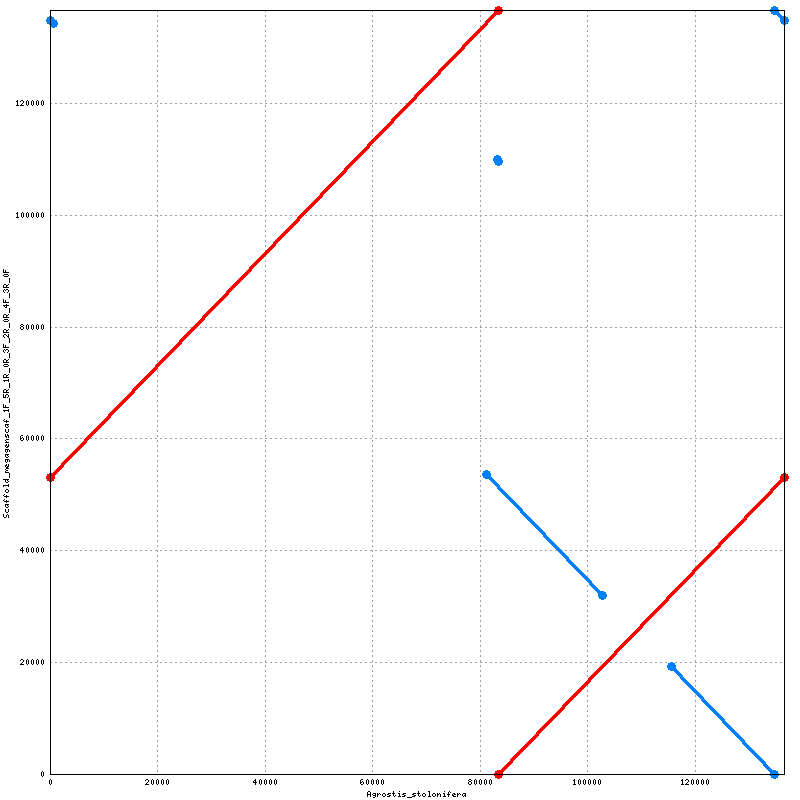
\includegraphics[scale=0.3]{dotplot_agro_wpm1}};
\node (wmp2) at (8,-7) {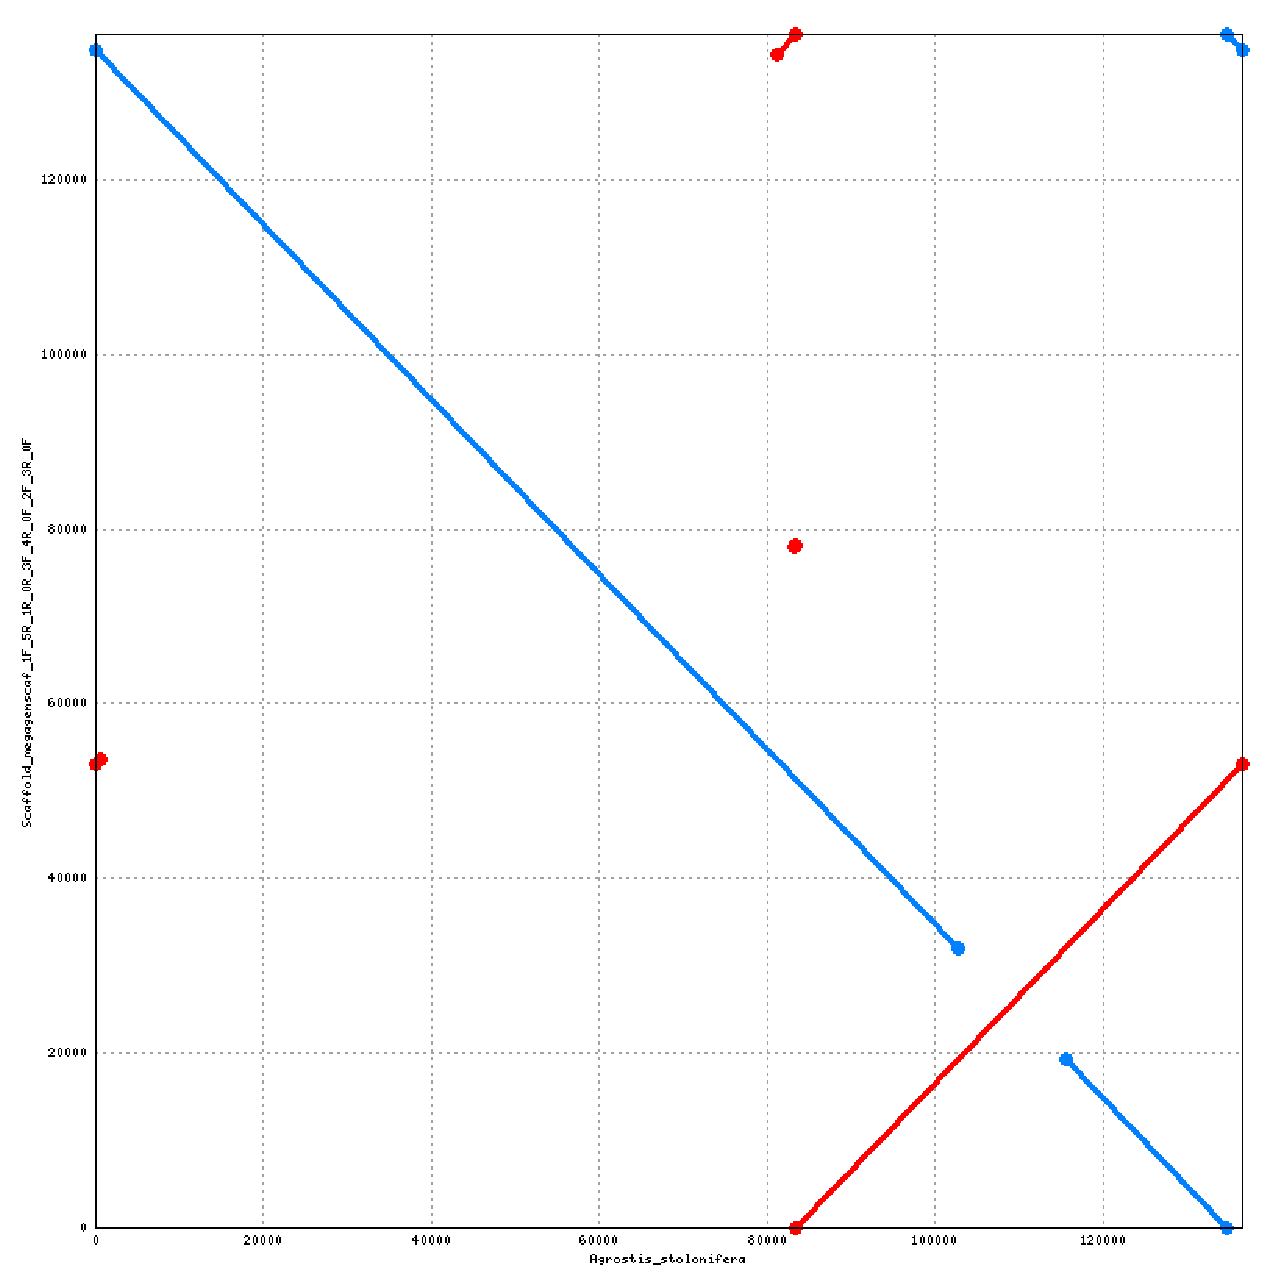
\includegraphics[scale=0.3]{dotplot_agro_wpm2}};
\node (ref) at (8,0) {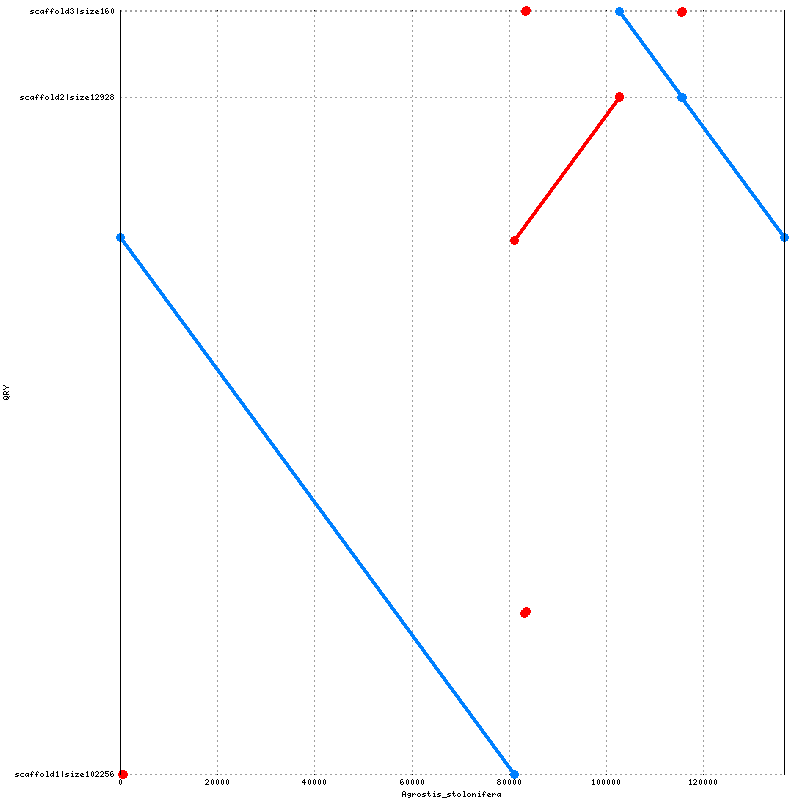
\includegraphics[scale=0.3]{dotplot_agro_sspace}};
\node (sspace) at (0,0) {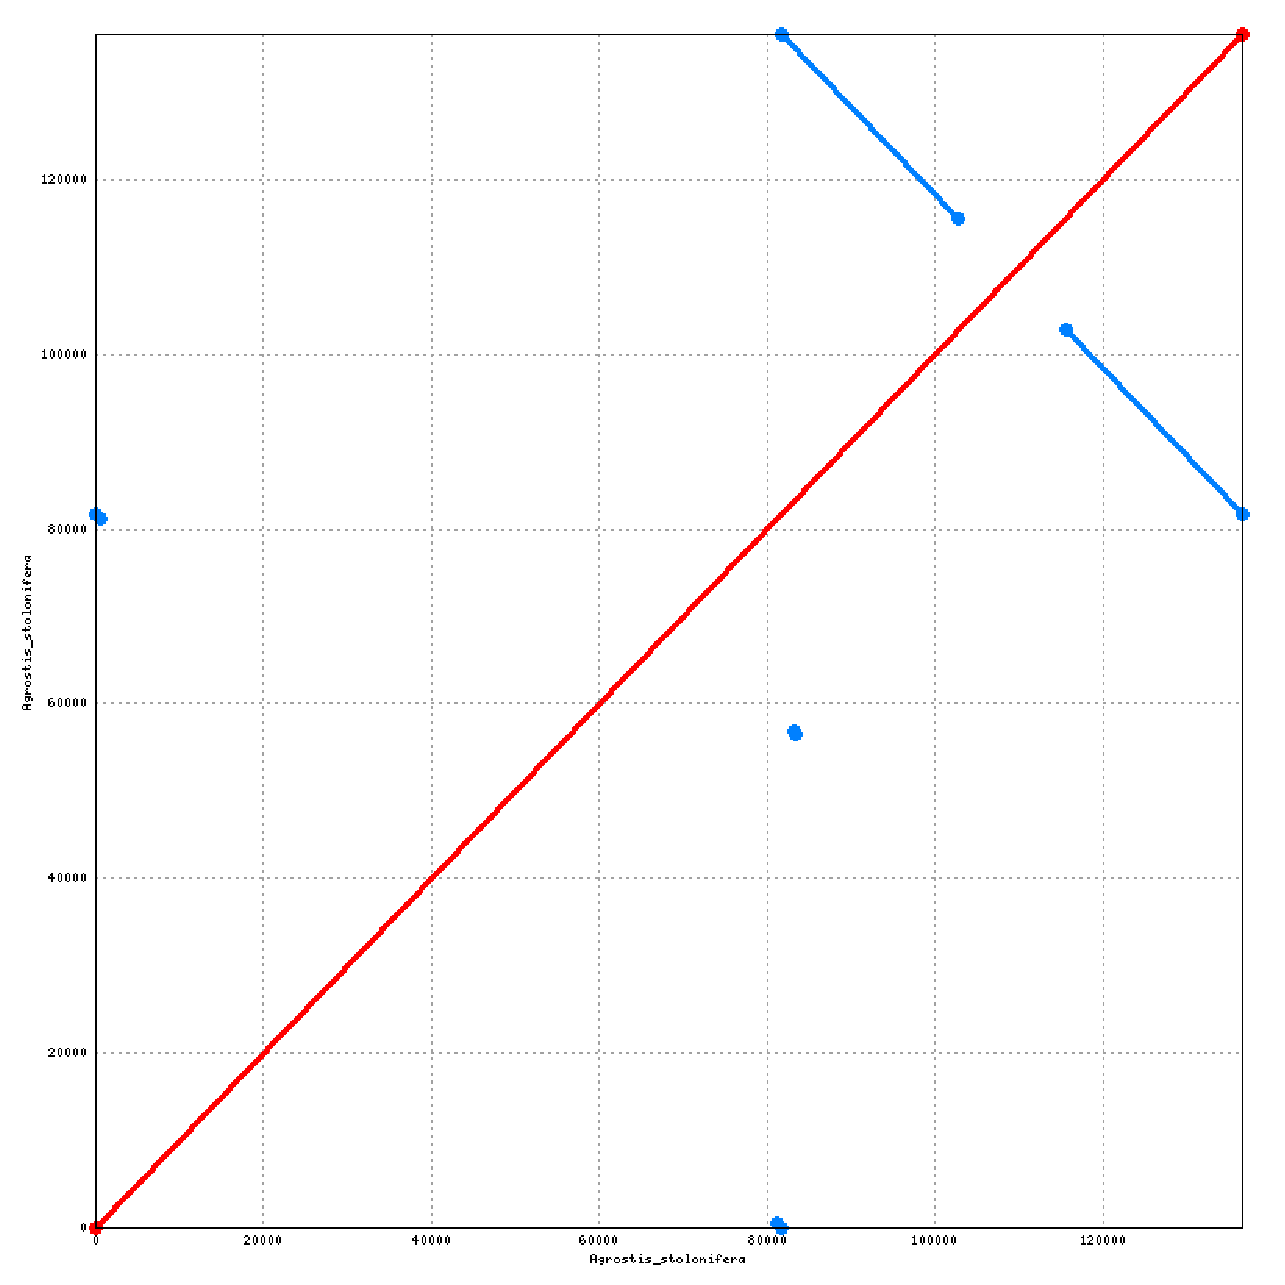
\includegraphics[scale=0.3]{dotplot_agrostis_agrostis}};
\end{tikzpicture}
}
\end{center}
\caption{Control dotplot and dotplots of weighted path model and SSPACE scaffolding solutions with the reference genome on the $x$ axis}
\footnotesize Control (top left), sspace (top right), wpm solutions (bottom). The control is the reference aligned to itself.\\ \texttt{> nucmer ref\_genome.fasta [solution, reference, unitigs] > align.delta} \\ \texttt{> mummerplot align.delta}
\label{dotplotsols}
\end{figure}

\clearpage
\subsubsection{Quality assessment of genome assemblies of \textit{Pinus koraiensis} chloroplastic genome}

\paragraph*{QUAST}
As a reminder, \textit{Pinus koraiensis} chloroplastic genome does not possess an inverted repeat. The genome is smaller than the average size for a chloroplatic genome. The pinus instance has 33 unitigs, among them only 10 are bigger than 1000bp. The input graph is shown in annexe \ref{fig:graphpinus}. This instance possesses many small repeats and is difficult to assemble. Some unitigs are as small as 76bp. Knowing that the contig builder \textsc{minia} built pinus unitigs with a k-mer size of 60, this is dissapointingly small, and smaller than the read size (150bp). These unitigs are solely linked by overlaps (as the chance of having a mated-pair on them is low, or null for unitigs smaller than the read size). Knowing these unitigs are repeats, their overlaps are hard to trust. \\
Pinus is never correctly solved by first generation GST (wpm and dist) and only partially solved by the first step of the flow model. Quast results suggests that the best assembly is obtained with SSPACE as there are only 2 misassemblies for a 99.254\% of assembled genome. However SSPACE assembles 12 large unitigs into a single scaffold then ignores all other unitigs (the remaining 21 which appear alone). SSPACE extends the unitigs through reads and uses 886 N to achieve the 99.254\% assembled genome score. This scaffold also contains two missassemblies, indels and mismatches. All these metrics are worse than those for the $1^{st}$ flow model step. \\ Only 1\% of the genome are repeats (unitig genome fraction $=99.079$). Wpm duplicates some contigs and achieves a 99.4\% score however has 11 misassemblies which is extremely disappointing. Hopes for the flow model are high despite it assembling only 92\% of the genome: it has the high NA50, meaning that for 96535 nucleotides the assembly is perfect. SSPACE's first missassembly occurs at the 86569bp. Nucmer alignements for these scaffolding solutions are shown in annexe \ref{fig:dotpinus}.
% PINUS TABLE MANNNN
\begin{table}[h!]
\scriptsize
\begin{center}
\resizebox{14cm}{!}{
\begin{tabular}{|l*{5}{|r}|}
\hline
Assembly & unitigs & flow\_step1\_sol & wpm\_sol1.fsa & sspace\_sol & ref\_genome \\ \hline
\# contigs ($\geq$ 0 bp) & 33 & 2 & {\bf 1} & 21 & {\bf 1} \\ \hline
\# contigs ($\geq$ 1000 bp) & 10 & {\bf 1} & {\bf 1} & {\bf 1} & {\bf 1} \\ \hline
Total length ($\geq$ 0 bp) & 118629 & 116214 & 116866 & {\bf 119654} & 116866 \\ \hline
Total length ($\geq$ 1000 bp) & 115186 & 115838 & 116866 & {\bf 117042} & 116866 \\ \hline
\# contigs & 11 & {\bf 1} & {\bf 1} & {\bf 1} & {\bf 1} \\ \hline
Largest contig & 20834 & 115838 & 116866 & {\bf 117042} & 116866 \\ \hline
Total length & 115888 & 115838 & 116866 & {\bf 117042} & 116866 \\ \hline
Reference length & 116866 & 116866 & 116866 & 116866 & 116866 \\ \hline
GC (\%) & 38.77 & 38.86 & 38.80 & 38.79 & 38.80 \\ \hline
Reference GC (\%) & 38.80 & 38.80 & 38.80 & 38.80 & 38.80 \\ \hline
N50 & 14862 & 115838 & 116866 & {\bf 117042} & 116866 \\ \hline
\# misassemblies & {\bf 0} & 1 & 11 & 2 & {\bf 0} \\ \hline
\# misassembled contigs & {\bf 0} & 1 & 1 & 1 & {\bf 0} \\ \hline
Misassembled contigs length & {\bf 0} & 115838 & 116866 & 117042 & {\bf 0} \\ \hline
\# local misassemblies & {\bf 0} & 4 & 4 & 5 & {\bf 0} \\ \hline
\# unaligned contigs & 0 + 0 part & 0 + 0 part & 0 + 0 part & 0 + 0 part & 0 + 0 part \\ \hline
Unaligned length & 0 & 0 & 0 & 0 & 0 \\ \hline
Genome fraction (\%) & 99.079 & 92.153 & 99.471 & 99.254 & {\bf 100.000} \\ \hline
Duplication ratio & 1.001 & 1.076 & 1.005 & 1.010 & {\bf 1.000} \\ \hline
\# N's per 100 kbp & {\bf 0.00} & 6997.70 & {\bf 0.00} & 757.85 & {\bf 0.00} \\ \hline
\# mismatches per 100 kbp & {\bf 0.00} & {\bf 0.00} & 5.16 & 0.86 & {\bf 0.00} \\ \hline
\# indels per 100 kbp & 2.59 & 1.86 & 8.60 & 2.59 & {\bf 0.00} \\ \hline
\# genes & 261 + 6 part & 249 + 4 part & 262 + 7 part & 262 + 6 part & {\bf 270 + 0 part} \\ \hline
Largest alignment & 20834 & 96535 & 28559 & 86569 & {\bf 116866} \\ \hline
NA50 & 14862 & 96535 & 20762 & 86569 & {\bf 116866} \\ \hline
\end{tabular}
}
\end{center}
\caption{QUAST metrics for several unitig scaffoldings of \textit{Pinus koraiensis} with GST (wpm, flow model) and SSPACE}
\footnotesize{All statistics are based on contigs of size $\geq$ 50 bp. {\color{magenta}wpm}: weighted path model, {\color{magenta}flow\_step1}: step 1 of flow model.}
\label{tab:pinus}
\end{table}



\clearpage
\subsection{Partially solved instance - flow model}\label{sec:wolbachia}
Wolbachia is partially assembled by the first step of the flow model. Table \ref{tab:insert} highlights the importance of correctly choosing the mated-pair reads' insert size. Results show a drastic improvement of the total assembled length when changing the mate paired insert size from 1000bp to 2000bp. This length gradually decreases as the insert size increases (same with the genome size metric). One proposed explanation is the repeats' sequence size of \textit{Wolbachia Endosymbiont}. As previously seen in figure \ref{fig:wolbarepeats}, the bacterial genome has repeats with sizes mainly between 500bp and 1.2Kbp. These repeats are partially solved during the unitig building step. The issue comes from genomically close repeats bigger than 1.2Kbp. There are 25 repeats of this type, among them 3 bigger than 5kbp. The location of these repeats coincide with regions of major scaffolding problems, where unitigs are not scaffolded or so badly scaffolded that they do not map on the reference genome. To see the exact coordinates of those location see annexe \ref{tab:repeatcoord}. The insert size must be big enough to overlap all repeats however increasing the insert size too much impacts on the scaffolders' ability to precisely join regions containing smaller repeats. Using multiple libraries would be a solution however this strategy didn't result in encouraging scaffolding solutions with SSPACE (library i2000 and i5000 used simultaneously). Another interesting metric to notice is the genome fraction covered by unitigs, which is very low (90.3\%) considering that the genome is 1.4Mbp and repeats rarely exceed 1.2Kb . This is also noticeable in figure \ref{fig:alignwoinsert}, where rather large portions of the reference genome are not covered by unitigs. The unitig building step failed to produce large sequences covering these areas because they contain many very small ($\leq$ read size) tandem repeats. Unless filled with Ns, these areas will never be scaffolded. Obtaining a whole circular genomes appears to be a very difficult task, but obtaining larger scaffolds should be possible.

\begin{table}[ht]
\begin{center}
\resizebox{18cm}{!}{
\begin{tabular}{|l*{13}{|r}|}
\hline
Assembly & unitigs & wolba\_i10k & wolba\_i11k & wolba\_i1k & wolba\_i2k & wolba\_i3k & wolba\_i4k & wolba\_i5k & wolba\_i6k & wolba\_i7k & wolba\_i8k & wolba\_i9k & ref\_genome \\ \hline
\# scaffolds ($\geq$ 0 bp) & 444 & 9 & 7 & 37 & 28 & 19 & 13 & 13 & 13 & 11 & 9 & 9 & {\bf 1} \\ \hline
\# scaffolds ($\geq$ 1000 bp) & 138 & 9 & 7 & 37 & 28 & 19 & 13 & 13 & 13 & 11 & 9 & 9 & {\bf 1} \\ \hline
Total length ($\geq$ 0 bp) & 1364357 & 871378 & 847704 & 615455 & 1214243 & 1197652 & 1121566 & 1101921 & 1084716 & 1045627 & 869142 & 879828 & {\bf 1482355} \\ \hline
Total length ($\geq$ 1000 bp) & 1290990 & 871378 & 847704 & 615455 & 1214243 & 1197652 & 1121566 & 1101921 & 1084716 & 1045627 & 869142 & 879828 & {\bf 1482355} \\ \hline
\# scaffolds & 444 & 9 & 7 & 37 & 28 & 19 & 13 & 13 & 13 & 11 & 9 & 9 & {\bf 1} \\ \hline
Largest scaffolds & 87315 & 387284 & 387518 & 63122 & 222630 & 368628 & 368594 & 483412 & 211466 & 334472 & 249957 & 249957 & {\bf 1482355} \\ \hline
Total length & 1364357 & 871378 & 847704 & 615455 & 1214243 & 1197652 & 1121566 & 1101921 & 1084716 & 1045627 & 869142 & 879828 & {\bf 1482355} \\ \hline
Reference length & 1482355 & 1482355 & 1482355 & 1482355 & 1482355 & 1482355 & 1482355 & 1482355 & 1482355 & 1482355 & 1482355 & 1482355 & 1482355 \\ \hline
GC (\%) & 34.01 & 33.92 & 33.94 & 34.08 & 33.89 & 33.95 & 33.96 & 33.96 & 33.91 & 33.93 & 33.95 & 33.94 & 34.19 \\ \hline
Reference GC (\%) & 34.19 & 34.19 & 34.19 & 34.19 & 34.19 & 34.19 & 34.19 & 34.19 & 34.19 & 34.19 & 34.19 & 34.19 & 34.19 \\ \hline
N50 & 17458 & 142935 & 143187 & 21300 & 68630 & 75831 & 142496 & 122998 & 116953 & 189499 & 189823 & 189972 & {\bf 1482355} \\ \hline
NG50 & 14993 & 68085 & 68090 & - & 59359 & 69791 & 122971 & 77779 & 93415 & 122899 & 45001 & 57433 & {\bf 1482355} \\ \hline
\# misassemblies & {\bf 0} & 1 & {\bf 0} & 12 & 3 & 1 & 1 & {\bf 0} & {\bf 0} & {\bf 0} & 1 & {\bf 0} & {\bf 0} \\ \hline
\# misassembled scaffolds & {\bf 0} & 1 & {\bf 0} & 7 & 3 & 1 & 1 & {\bf 0} & {\bf 0} & {\bf 0} & 1 & {\bf 0} & {\bf 0} \\ \hline
Misassembled scaffolds length & {\bf 0} & 142935 & {\bf 0} & 139698 & 143728 & 22037 & 35610 & {\bf 0} & {\bf 0} & {\bf 0} & 142540 & {\bf 0} & {\bf 0} \\ \hline
\# local misassemblies & {\bf 0} & 23 & 23 & 45 & 66 & 60 & 52 & 47 & 42 & 38 & 30 & 26 & {\bf 0} \\ \hline
\# unaligned scaffolds & 0 + 0 part & 0 + 0 part & 0 + 0 part & 0 + 0 part & 0 + 0 part & 0 + 0 part & 0 + 0 part & 0 + 0 part & 0 + 0 part & 0 + 0 part & 0 + 0 part & 0 + 0 part & 0 + 0 part \\ \hline
Unaligned length & 0 & 0 & 0 & 0 & 0 & 0 & 0 & 0 & 0 & 0 & 0 & 0 & 0 \\ \hline
Genome fraction (\%) & 90.341 & 53.726 & 51.551 & 40.034 & 78.587 & 76.826 & 71.970 & 70.313 & 68.955 & 66.047 & 54.424 & 54.992 & {\bf 100.000} \\ \hline
Duplication ratio & 1.019 & 1.094 & 1.109 & 1.040 & 1.042 & 1.052 & 1.051 & 1.057 & 1.061 & 1.068 & 1.077 & 1.079 & {\bf 1.000} \\ \hline
\# N's per 100 kbp & {\bf 0.00} & 8603.27 & 9854.62 & 1808.26 & 3969.22 & 4880.30 & 4859.72 & 5402.66 & 5764.55 & 6364.03 & 7177.65 & 7348.94 & {\bf 0.00} \\ \hline
\# mismatches per 100 kbp & {\bf 0.00} & {\bf 0.00} & {\bf 0.00} & 42.97 & {\bf 0.00} & {\bf 0.00} & {\bf 0.00} & {\bf 0.00} & {\bf 0.00} & {\bf 0.00} & {\bf 0.00} & {\bf 0.00} & {\bf 0.00} \\ \hline
\# indels per 100 kbp & {\bf 0.00} & {\bf 0.00} & {\bf 0.00} & 4.72 & 0.09 & 0.09 & {\bf 0.00} & {\bf 0.00} & {\bf 0.00} & {\bf 0.00} & {\bf 0.00} & {\bf 0.00} & {\bf 0.00} \\ \hline
Largest alignment & 87315 & 356813 & 356813 & 62424 & 219709 & 359164 & 359164 & 459850 & 205359 & 319611 & 237693 & 237693 & {\bf 1482355} \\ \hline
NA50 & 17458 & 89651 & 115294 & 16288 & 59479 & 71508 & 134513 & 111512 & 111512 & 116821 & 99293 & 119120 & {\bf 1482355} \\ \hline
NGA50 & 14993 & 23733 & 29168 & - & 51212 & 64638 & 71508 & 56028 & 74077 & 56028 & 33486 & 44273 & {\bf 1482355} \\ \hline
\end{tabular}
}
\end{center}
\caption{Scaffolding solutions of the flow model step 1 with mated-pair reads libraries of different insert sizes compared to the reference genome and the initial unitig set.}
\footnotesize All statistics are based on contigs of size $\geq$ 50 bp. \\
Wolbachia has 444 unitigs, among them 306 are smaller than 1000bp. In this comparison, the higher the number of scaffolds the better because it indirectly depicts the number of unitigs the $1^{st}$ step of the flow model considers as big unitigs. It impacts the total length of the assembled genome which is the largest with an insert size of 2000bp (1.2Mbp). The largest perfect alignement found is with an insert size of 5000bp (459Kb) indicating this insert size is the upper limit to use for wolbachia. For all solutions the number of missassemblies is very high due to the fact that they are heavily gapped and the gap size not exact or unknown. 
\label{tab:insert}
\end{table}

Figure \ref{fig:alignwoinsert} shows the alignement of all scaffolding strategies tested for wolbachia to the reference genome. Additionally the unitigs were also aligned to the reference genome to highligh the uncovered 350Kbp - 500Kbp and 1380Kpb - 1440Kpb regions. SSPACE solution with the 2Kbp insert size library shows the less misassembled regions with the most reference coverage however this scaffolder still has more misassembled regions than the worst of the flow model solutions. At the end of the SSPACE scaffolding process, there are 338 separate scaffolds left (not shown). This means small unitigs were not used and SSPACE mainly extended big existing unitigs with reads. SSPACE also fails to produce any valid scaffold for the genomic regions containing the large ($>$Kbp) repeats (see their exact coordinates in annexe \ref{tab:repeatcoord}).
\begin{figure}[h!]
\begin{center}
\resizebox{18cm}{!}{
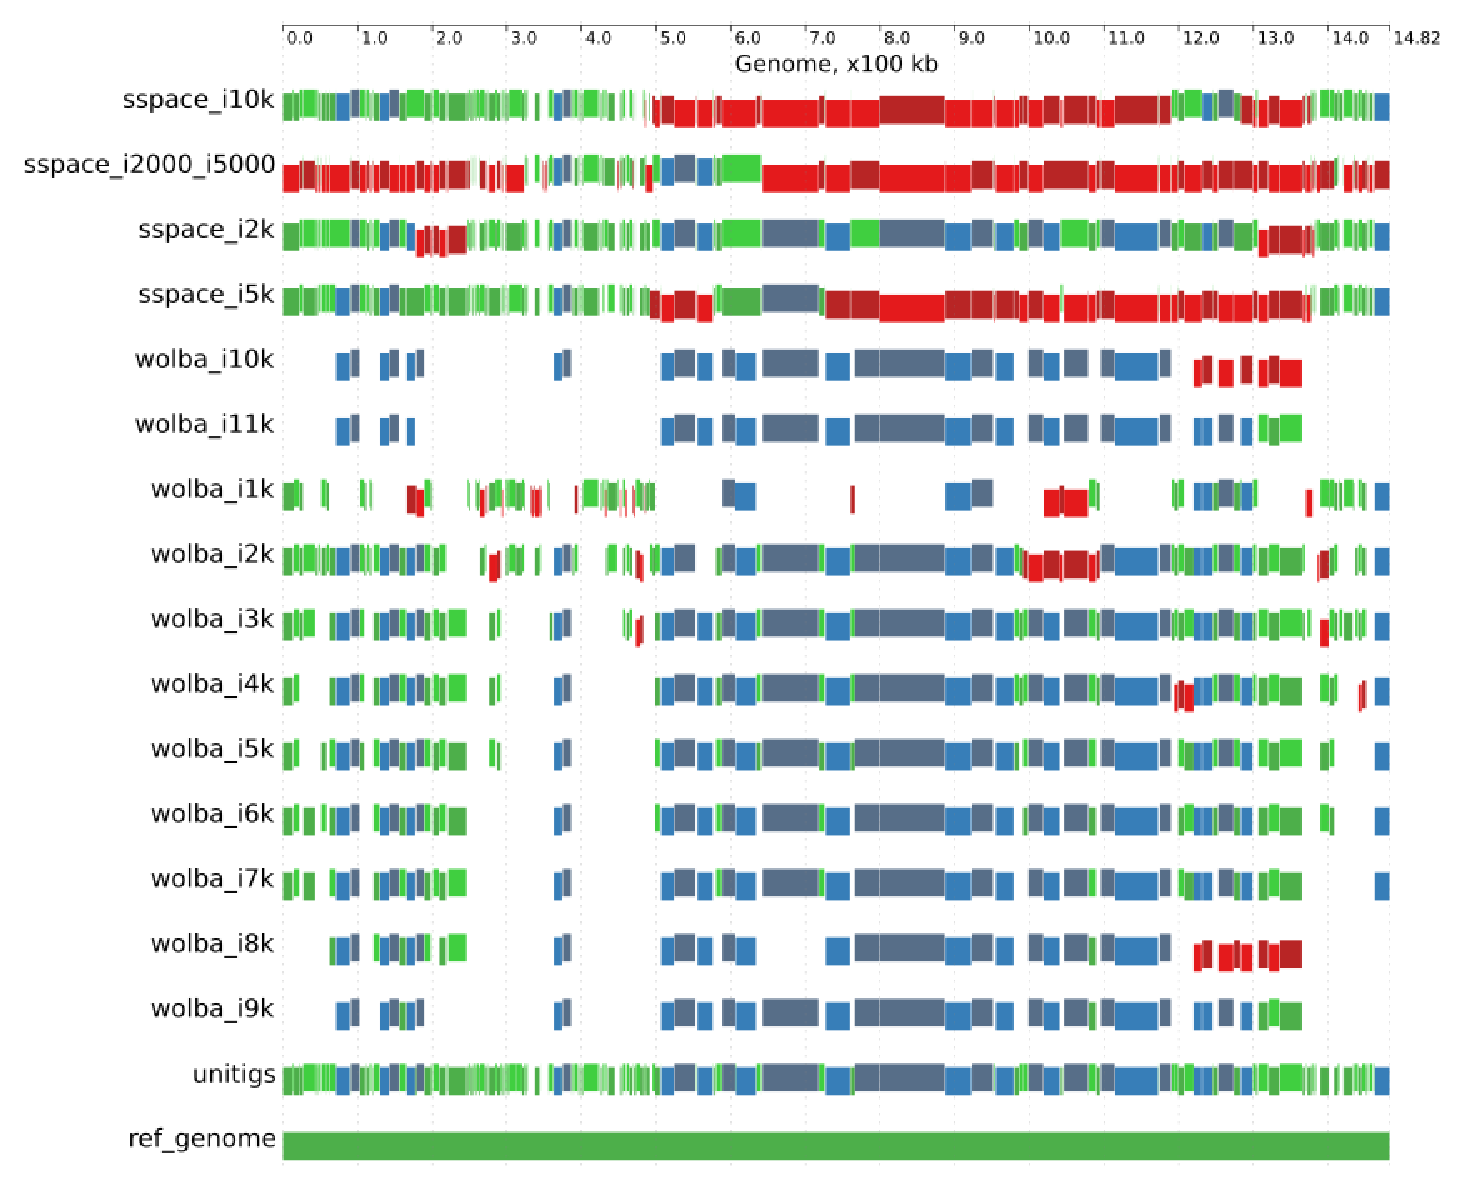
\includegraphics[scale=0.7]{alignment_woinserts}
}
\end{center}
\caption{Alignment of scaffolding solutions on the reference genome of \textit{Wolbachia endosymbiont}}
\scriptsize This plot shows alignment of unitigs or scaffolds to the reference genome and positions of misassemblies in the scaffolds. Correctly aligned big ($>$ 10kb) scaffolds are blue if the boundaries are exact, and green if the boundaries are different from the reference genome region it was mapped to. Scaffolds containing an important amount of misassemblies are red.
\label{fig:alignwoinsert}
\end{figure}

The repeated unitigs should be introduced in the $2^{nd}$ step of the flow model. The fraction of the assembled genome should be at least as good as SSPACE. The strategy used for this second step will decide if the order and orientation will be satisfactory. As of now, two strategies are considered. The first is an interative gap by gap approach, which is faster but whose solution depends heavily of the order in which the gaps are treated. The second approach is filling all gaps at once. This approach seems more sensible but will result in a combinatorial problem with many possible solutions, especially since gaps are distance intervals. 

\clearpage
%-------------------------------------------------------------------------------
% BODEH!
%-------------------------------------------------------------------------------
\section{Conclusion} \label{sec:conc}
The \textsc{Genscale} scaffolding methodology basis is the computing and pre-processing of unitig coverage. Different modeling strategies are tested and evaluated to solve the scaffolding problem. Adding weight on links to model the distance between unitigs does not lead to better results. These additional constraints are too demanding. An evaluation strategy was set up to understand why some data sets are especially challenging. The repeat content impacting on the unitig number rather than the size of the genome is the cause of complex input data. Some explanations are provided for problematic data sets (disconnected graph or missing link) however the main source of difficulties is the size of the modeled graph. A new two step scaffolding modeling strategy is in development. It tries to break the graph complexity by first solving a graph containing only large unitigs - building something that can be compared to a trustworthy genomic frame. The benchmarking workflow brings together several sequence comparing tools: a tool for assessing assembly quality (Quast), a sequence aligner (MUMmer) and homemade visualization and comparison scripts (\texttt{graph\_generator.py} and \texttt{graph\_comparato.py}). Although compared to a single published scaffolder (SSPACE), this methodology can be applied for any scaffolding solution obtained with other tools. Comparing the GST to recent publications such as the ScaffMatch\cite{mandric_scaffmatch:_2015} scaffolder or the Integer Linear Programming approach\cite{ilp_montpellier} developed at the Montpellier Laboratory of Informatics, Robotics and Microelectronics (LIRMM) which explicitly discusses its repeated sequence processing will be insightful. Their article was the motivation behind the study on \textit{Wolbachia Endosymbiont}, one of their tested organism. The benchmarking of the GST highlights the major advantage of processing unitig coverage but also the limitation of the models which have difficulties with bigger graphs with high degree nodes. Overall the project succeeded more in the standardisation of evalution and benchmarking strategies than on providing precise explanations for unsuccessful scaffoldings. The immediate perspective is to help guide the development of the flow model.

\section*{Future applications}\label{sec:persp}
Genome sequencing is currently undergoing another transition from Illumina type short-read NGS to long-read sequencing technologies. Sometimes called "Third Generation Sequencing", long-read sequencing technologies were launched a few years ago. One of these technologies is the Oxford Nanopore sequencer MinION \cite{ashton_minion_2015, madoui_genome_2015}. It can directly read a single DNA molecule and provide a more precise view of complex genomic organization and content - this should solve the assembly problems caused by short reads supposed to uniquely represent a portion of the genome. As shown in this report, this is rarely the case, and despite attempting to bypass the repeat issue by using unitigs and computing their coverage, the unreliable contradictory linking information persists. Regions containing short repeats are close to impossible to assemble and scaffold using short-read technologies. Yet repeated regions are often biologically very relevant. In microbes, short-sequence DNA repeats enable genetic flexibility \cite{van_belkum_short-sequence_1998}, often contain host-interacting genes and horizontally aquired coding regions \cite{wiedenbeck_origins_2011}. Long-read technologies do not have a great accuracy however, sometimes containing up to 30\% of sequencing errors. Correcting long MinION reads with high confidence Illumina short-reads is a proposed strategy to obtain quality longer reads, providing larger contigs and solving the repeat challege faced by scaffolding. Conducting a study on such data is an interesting prospect for scaffolders developed at \textsc{Genscale}.

\clearpage

%-------------------------------------------------------------------------------
%BIBLIOGRAPHY
%-------------------------------------------------------------------------------
\pagenumbering{gobble}
\bibliography{scaffoldingbiblio}
\bibliographystyle{naturemag}
%\printbibliography

\newpage
\section*{Annexes}
\label{sec:anx}
\setcounter{figure}{0}
\renewcommand{\thefigure}{\Alph{figure}}
\floatstyle{plaintop}
\restylefloat{figure}
\restylefloat{table}
%\renewcommand{\thetable}{\Alph{table}}

\begin{figure}[h!]
\caption{Input graph of pinus}
\footnotesize This graph is a graphical transcription of the \textit{.txt} input file of pinus. The graph as modeled by GST is by far bigger. Here we see several self-loops and multiple equivalent links (see 3 identical links between unitig 30 and unitig 7). These will be merged once the GST models the problem. A strategy would be to keep the link coverage as additional constrains to hopefully help find the optimal path. Most of the contigs are shorter than 1000bp (22) and some as small as 76bp. Knowing that the contig builder \textsc{minia} built pinus unitigs with a k-mer size of 60, this is dissapointingly small, and smaller than the read size (150bp). These unitigs are solely linked by overlaps (as the chance of having a mated-pair on them is low, or null for unitigs smaller than the read size). Knowing these unitigs are repeats, their overlaps are hard to trust \ldots
\label{fig:graphpinus}
\begin{center}
\resizebox{18cm}{!}{
\begin{tikzpicture}
\node (ref) at (0,0) {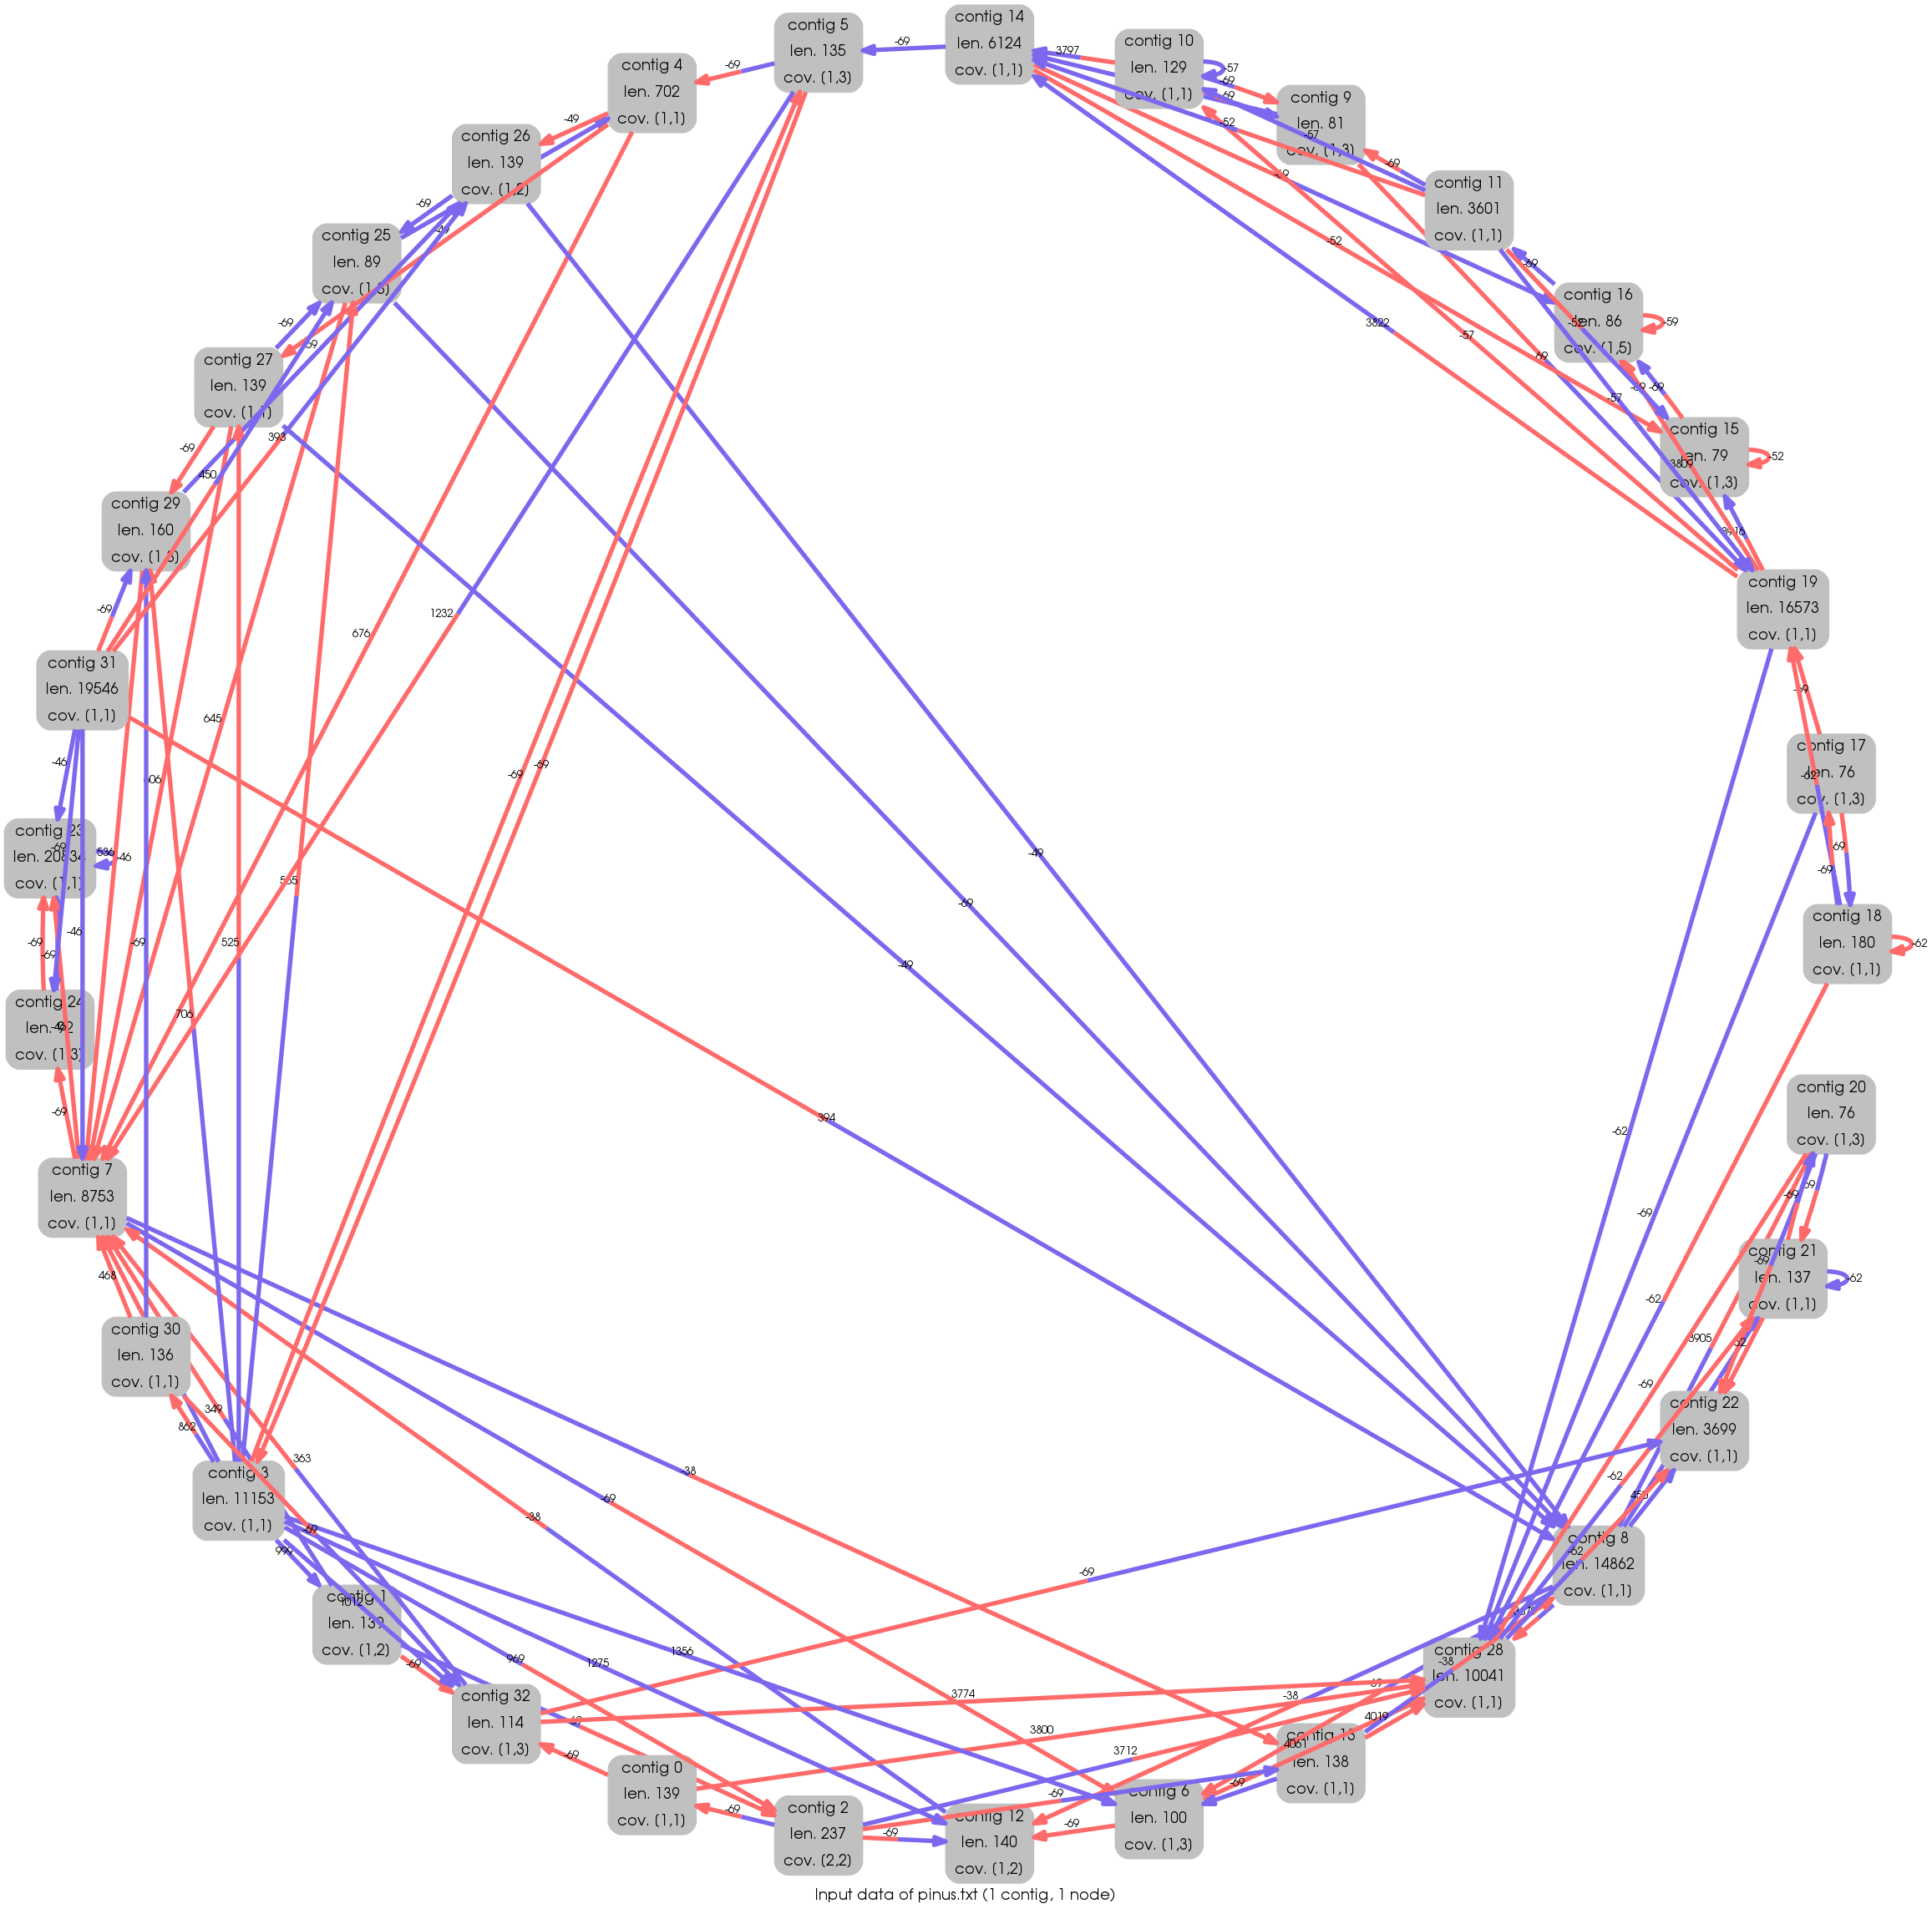
\includegraphics[scale=0.3]{pinustxt_solnr_0_INPT}};
\end{tikzpicture}
}
\end{center}
\end{figure}

\begin{figure}[h!]
\caption{Dotplots of weighted path model, $1^{st}$ flow model step and SSPACE scaffolding solutions with the reference genome on the $x$ axis}
\footnotesize Top left graph is the SSPACE solution, top right the flow model solution and bottom left the weighted path solution. The weighted path solution single scaffold contains many misassemblies - a lot of unitigs are scaffolded in the wrong order and orientation. The SSPACE solution contains many scaffolds because it did not scaffold small unitigs (overlapping unitig names on the left top of the graph). SSPACE extended the big unitigs and introduced Ns to be able to built the big scaffold matching the reference genome - though it contains misassemblies, mismatches and indels visualized as buldges (or little circles) on the main red matching line. The flow model dotplot also shows an almost perfect match, with gaps to be filled in with the second step of the model. The aim is to obtain a scaffold with less N and errors than SSPACE, as well as a better genome assembled fraction. 
\begin{center}
\label{fig:dotpinus}
\resizebox{18cm}{!}{
\begin{tikzpicture}
\node (wpm1) at (0,-7) {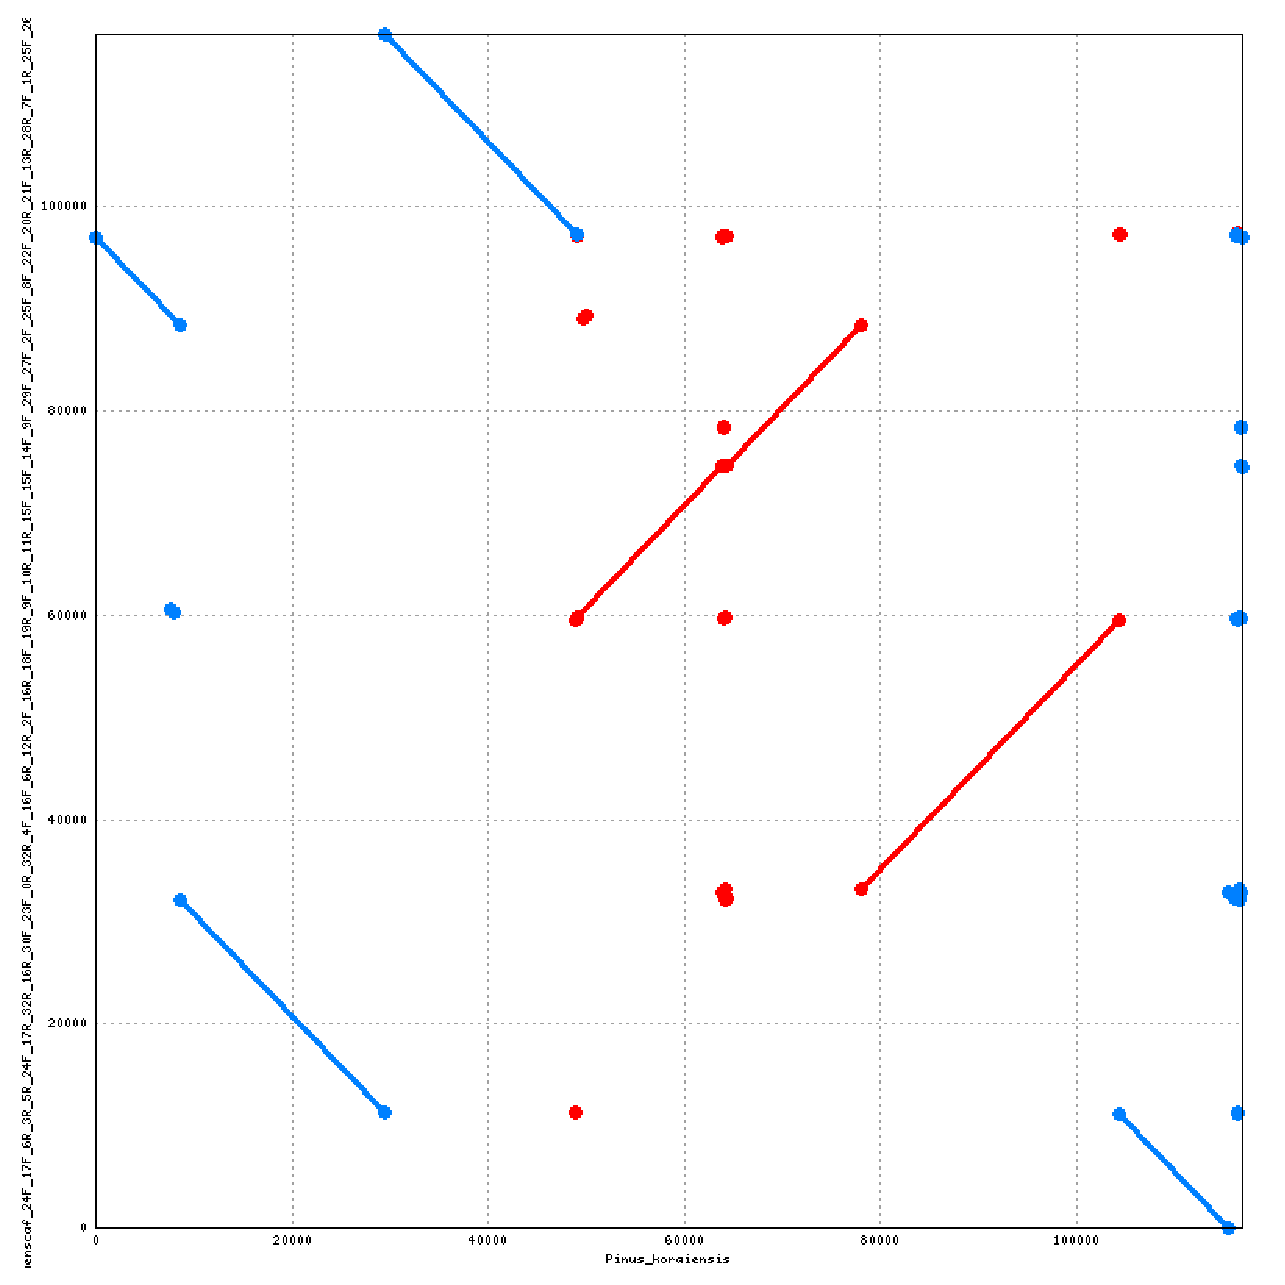
\includegraphics[scale=0.3]{pinus_vs_wpm}};
\node (wmp2) at (8,0) {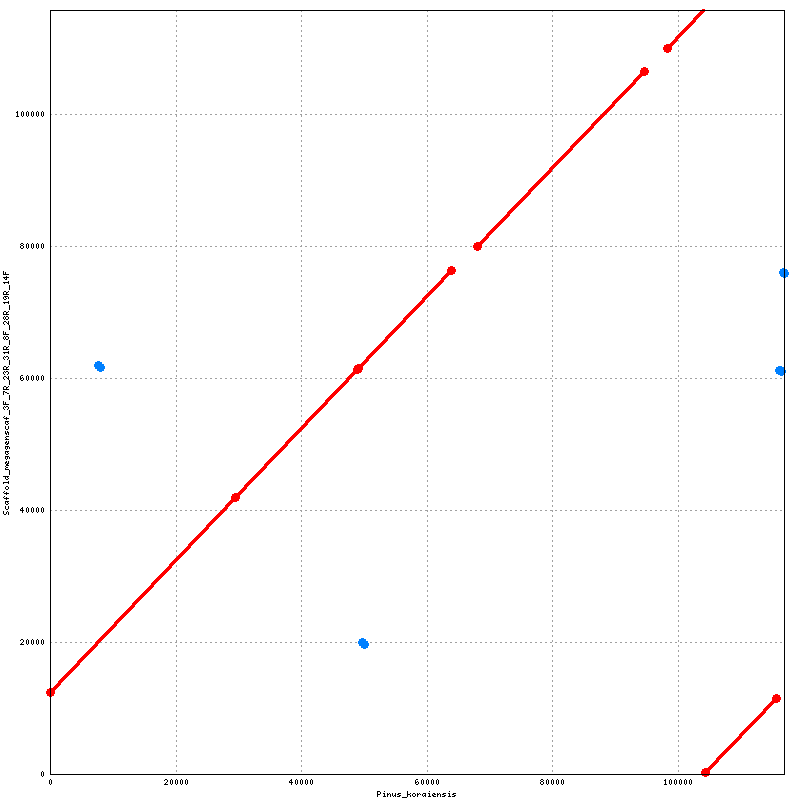
\includegraphics[scale=0.3]{pinus_vs_flow}};
\node (ref) at (0,0) {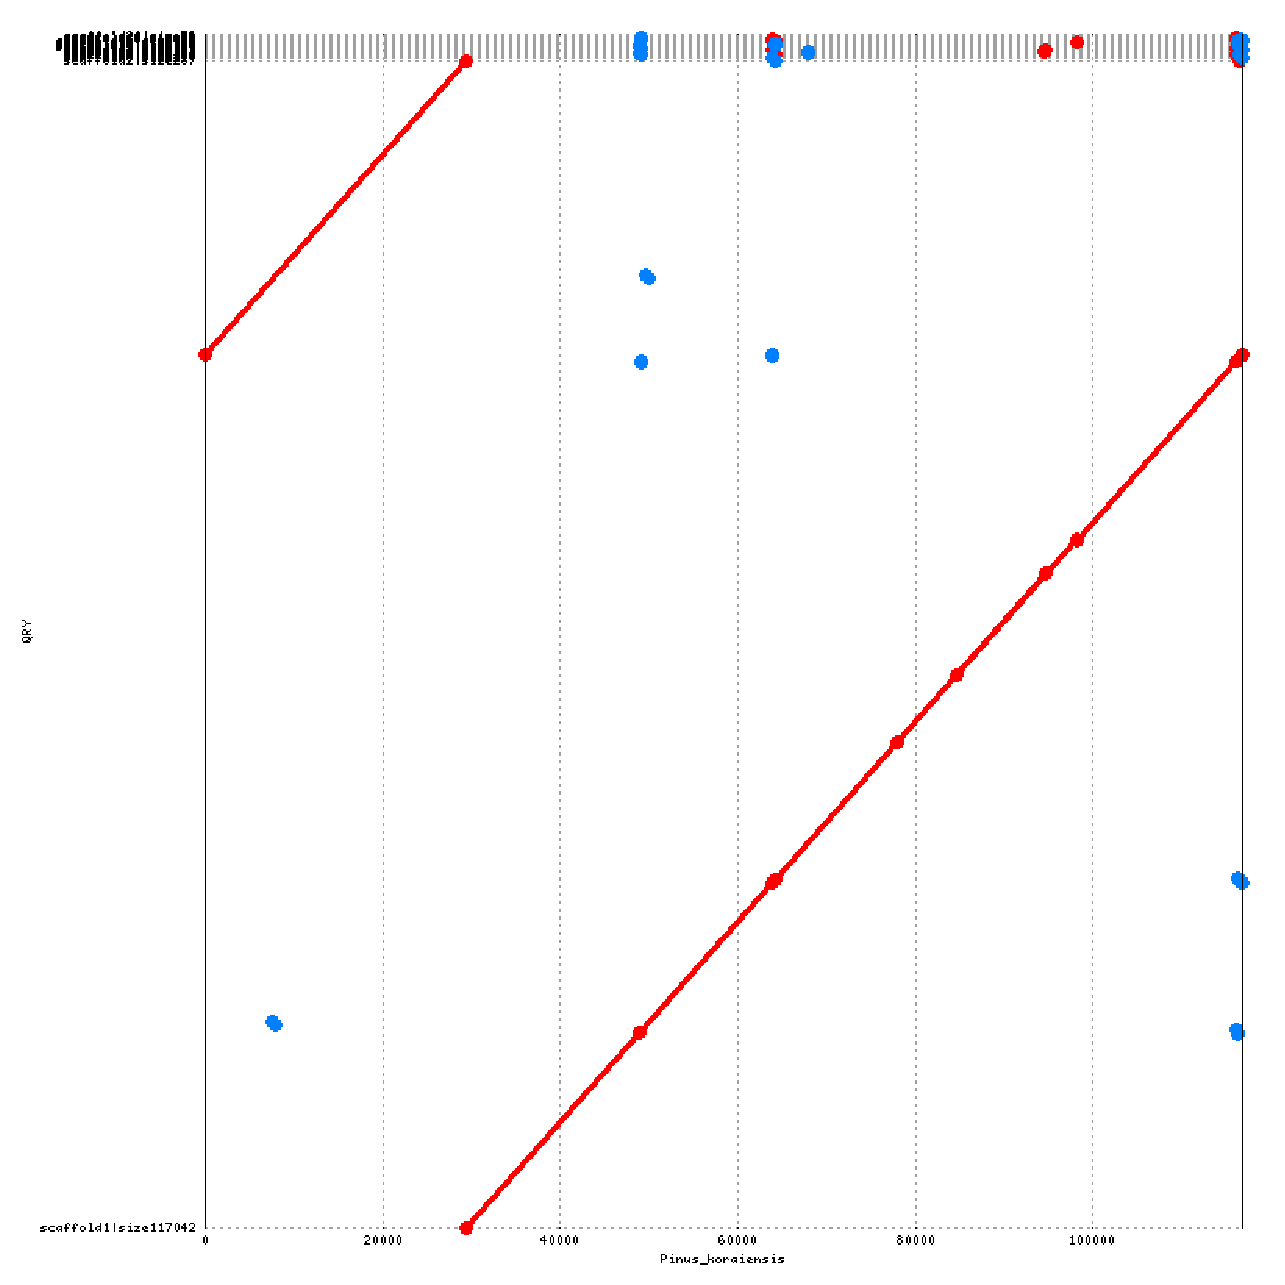
\includegraphics[scale=0.3]{pinus_vs_sspace_rev}};
\end{tikzpicture}
}
\end{center}
\end{figure}

\begin{figure}[h!]
\caption{Coordinates and length of repeats longer than 1.2Kbp in the \textit{Wolbachia endosymbiont} genome}
\footnotesize Obtained with the \texttt{show-coord} tool of the MUMmer software after the \texttt{nucmer} alignement of the reference genome to itself. Colored rows are coordinates of repeats longer than 2Kbp.\\
\textit{\color{magenta} S1}: start coordinate of sequence of $x$ axis \\
\textit{\color{magenta} E1}: end coordinate of sequence of $x$ axis \\
\textit{\color{magenta} S2}: start coordinate of sequence of $y$ axis (here, same sequence, the reference genome)\\
\textit{\color{magenta} E2}: end coordinate of sequence of $y$ axis (here, same sequence, the reference genome)\\
\textit{\color{magenta} LEN}: length of the matched region \\
\textit{\color{magenta} IDY}: indentity percentage of the matched region \\

\label{tab:repeatcoord}

\centering
\resizebox{12cm}{!}{
\begin{tabular}{|l|l|l|l|l|l|l|}
\hline
{[}S1{]} & {[}E1{]} & {[}S2{]} & {[}E2{]} & {[}LEN 1{]} & {[}LEN 2{]} & {[}\% IDY{]}  \\ \hline
1        & 1482355  & 1        & 1482355  & 1482355     & 1482355     & 100.00        \\
118235   & 119770   & 14639    & 13104    & 1536        & 1536        & 99.67          \\
951662   & 953006   & 62728    & 61384    & 1345        & 1345        & 100.00         \\
13104    & 14639    & 119770   & 118235   & 1536        & 1536        & 99.67          \\
295130   & 296467   & 156339   & 155002   & 1338        & 1338        & 100.00         \\
1044418  & 1046269  & 178963   & 177112   & 1852        & 1852        & 100.00         \\
295131   & 296471   & 201307   & 199967   & 1341        & 1341        & 99.93          \\
\rowcolor{red!10}
346054   & 354494   & 259128   & 250682   & 8441        & 8447        & 99.56          \\
1040287  & 1042282  & 286820   & 284825   & 1996        & 1996        & 100.00        \\
1370666  & 1372235  & 293326   & 291757   & 1570        & 1570        & 99.87          \\
886392   & 887730   & 296467   & 295129   & 1339        & 1339        & 100.00         \\
\rowcolor{red!10}
1459215  & 1461421  & 296650   & 294476   & 2207        & 2175        & 98.50          \\
\rowcolor{red!10}
353564   & 355681   & 325239   & 323122   & 2118        & 2118        & 97.54          \\
\rowcolor{red!10}
346054   & 351130   & 332648   & 327572   & 5077        & 5077        & 99.94          \\
\rowcolor{red!10}
250682   & 259128   & 354494   & 346054   & 8447        & 8441        & 99.56          \\
295130   & 296467   & 426552   & 425215   & 1338        & 1338        & 100.00         \\
\rowcolor{red!10}
353564   & 355681   & 449855   & 447738   & 2118        & 2118        & 97.54          \\
951661   & 953011   & 506502   & 505152   & 1351        & 1351        & 99.93          \\
1305338  & 1306686  & 553913   & 552565   & 1349        & 1349        & 99.93          \\
295129   & 296467   & 887730   & 886392   & 1339        & 1339        & 100.00         \\
505152   & 506502   & 953011   & 951661   & 1351        & 1351        & 99.93          \\
284825   & 286820   & 1042282  & 1040287  & 1996        & 1996        & 100.00         \\
177112   & 178963   & 1046269  & 1044418  & 1852        & 1852        & 100.00         \\
1334495  & 1335840  & 1306687  & 1305342  & 1346        & 1346        & 100.00         \\
1305342  & 1306686  & 1320819  & 1319475  & 1345        & 1345        & 100.00         \\
1305342  & 1306687  & 1335840  & 1334495  & 1346        & 1346        & 100.00         \\
291757   & 293326   & 1372235  & 1370666  & 1570        & 1570        & 99.87          \\
\rowcolor{red!10}
294476   & 296650   & 1461421  & 1459215  & 2175        & 2207        & 98.50         \\ \hline
\end{tabular}
}
\end{figure}


\clearpage
\begin{center}
\textsc{\Large Bioinformatics and Genomics Master's Degree\\ University Rennes 1}\\
\vspace*{0.1cm}
\textsc{Alexandrina Bodrug - June 22, 2015} \\
\vspace*{0.5cm}
\textsc{Genscale - Irisa}
\end{center}
\vspace*{2cm}
\paragraph*{Abstract [eng]} \textit{Next Generation Sequencing, scaffolding strategy, repeated sequence, data complexity assessment, benchmarking} \\
The last step of the NGS data assembling process is scaffolding - the ordering and relative orientation of large genomic sequences called contigs. The scaffolding process remains a challenging computational work because of the possible errors of NGS data and the intrinsic characteristics of genomes, such as repeated regions. The \textsc{Genscale} team develops new scaffolding methodologies which rely on contig coverage to solve the scaffolding problem of highly repeated genomes. The detection, processing and integration of repeated sequences in the scaffolding solution is a defining feature of these methodologies. This report describes the strategies used for benchmarking these tools with published scaffolders and the evaluation of the solutions found given the known input data and the expected solution. The data used for this project is simulated from small genomes containing many repeats - namely chloroplastic genomes and bacterial genomes. Limits and ways to optimise the \textsc{Genscale} scaffolders are outlined.

\vspace*{0.5cm}
\selectlanguage{french}
\paragraph*{Résumé [fr]} \textit{Séquençage Haut Débit, stratégie d'échafaudage, séquence répétée, estimation de la compléxité des données, analyse comparative}\\
La dernière étape du processus d'assemblage de données NGS est le scaffolding - l'ordonnancement et l'orientation relative de longues séquences génomiques appelées contigs. Le scaffolding est un processus difficile à cause d'erreurs possible dans les données NGS et des caractéristiques intrinsèques des génomes, telle que les régions répétées. L’équipe \textsc{Genscale} développe de nouvelles méthodologies de scaffolding qui se basent sur la couverture des contigs pour résoudre les problèmes de scaffolding posées par les génomes hautement répétés. La détection, le traitement et l'intégration des régions répétées dans la solution de scaffolding est une particularité de ces méthodologies. Ce rapport décrit les stratégies utilisées pour l'analyse comparative de ces outils avec des scaffoldeurs publiés et l'évaluation des solutions obtenues en connaissance de la nature des données en entrée et de la solution attendue. Les données utilisées dans ce projet sont simulées à partir de petits génomes contenant beaucoup de répétitions - à savoir des génomes chloroplastiques et des génomes bactériens. Sont également exposées dans ce rapport les limites et les possibilités d'optimisation des scaffoldeurs \textsc{Genscale}.

\end{document}